\documentclass[authoryear, 12pt]{elsarticle}

\usepackage{graphicx}
% \usepackage{lineno}
\usepackage{amssymb}
\usepackage{wrapfig}
\usepackage{subfig}
\usepackage{tipa}
\usepackage{float}

\journal{}

\begin{document}

\begin{frontmatter}

\title{The development of children's ability to track and predict turn structure in conversation}

\author[MPI]{Marisa Casillas\corref{cor1}}
\address[MPI]{Max Planck Institute for Psycholinguistics, Nijmegen}
%\address[StanfordLX]{Department of Linguistics, Stanford University}
\cortext[cor1]{Corresponding author}

\author[StanfordPSY]{Michael C. Frank}

\address[StanfordPSY]{Department of Psychology, Stanford University}

\begin{abstract}
We investigate language acquisition through the lens of a fundamental conversational skill: Turn taking. Children begin developing turn-taking skills in infancy, but take several years to assimilate their growing knowledge of language into their turn-taking behavior. In two eye-tracking experiments, with children across a wide developmental range, we measured spontaneous predictions about upcoming speaker change while controlling the amount of linguistic information available. We found that children already predicted upcoming turns at age one, but that they integrated linguistic cues differently at different ages. Children under three showed a general advantage for prosody over lexicosyntax, contrary to prior findings for adults. Children two and older showed more predictive switches for questions than non-questions, but only when lexical information was available. We found no evidence that lexicosyntax alone guides turn prediction---instead, participants' performance was best overall with access to lexicosyntax and prosody together. Our results point to the importance of studying children's linguistic processing in the context of conversation.
\end{abstract}

\begin{keyword}
Turn taking \sep Conversation \sep Development \sep Prosody \sep Lexical \sep Questions \sep Eye-tracking \sep Anticipation
%% MSC codes here, in the form: \MSC code \sep code
%% or \MSC[2008] code \sep code (2000 is the default)

\end{keyword}

\end{frontmatter}

% \linenumbers

\section{Introduction}
\label{sec:intro}

Spontaneous conversation is a universal context for using and learning language. Like other types of human interaction, it is organized at its core by the roles and goals of its participants. But what sets conversation apart is its structure: Sequences of interconnected, communicative actions that take place across alternating turns at talk. Sequential, turn-based structures in conversation are strikingly uniform across language communities and linguistic modalities. Turn-taking behaviors are also cross-culturally consistent in their basic features and the details of their implementation \citep{de-vos2015, dingemanse2013, stivers2009}. How does this ability develop? 

Children participate in sequential coordination with their caregivers starting at three months of age---before they can rely on any linguistic cues in taking turns \citep[see, among others, ][]{bateson1975, hilbrink2015, jaffe2001, snow1977}. Of course, infant turn taking is different from adult turn taking in several ways. Infant turn taking is heavily scaffolded by caregivers, has distinct timing in comparison to adult turn taking, and lacks semantic content \citep{hilbrink2015, jaffe2001}. However, children's early, turn-structured social interactions are presumably a critical precursor to their conversational turn taking. Along these lines, early non-verbal interactions establish the protocol by which children come to use language with others. And as they acquire language, they also come to integrate it into the preverbal turn-taking systems.

In this study, we investigate when children begin to make predictions about upcoming turn structure in conversation, and how they integrate language into their predictions as they grow older. In what follows, we first give a basic review of turn-taking research and the state of current knowledge about adult turn prediction. We then discuss recent work on the development of turn-taking skills before turning to the details of our own study.

\subsection{Turn taking}

Turn taking itself is not unique to conversation. Many other human activities are organized around sequential turns at action. Traffic intersections and computer network communication both use turn-taking systems. Children's early games (e.g., give-and-take, peek-a-boo) have built-in, predictable turn structure \citep{ratner1978, ross1987}. Even monkeys take turns: Non-human primates such as marmosets and Campbell's monkeys vocalize contingently with each other in both natural and lab-controlled environments \citep{lemasson2011, takahashi2013}. In all these cases, turn taking serves as a protocol for interaction, allowing the participants to coordinate with one another through sequences of contingent action. 

Conversation distinguishes itself from non-conversational turn-taking behaviors by the complexity of the turn sequencing involved. In the examples above (traffic, games, and monkeys) the set of sequence and action types is far more limited and predictable than what we find in everyday talk. For example, conversational turns come grouped into semantically-contingent sequences of action. The groups can span turn-by-turn exchanges (e.g., simple question--response, ``How are you?''--``Fine.'') or sequence-by-sequence exchanges (e.g., reciprocals, ``How are you?''--``Fine, and you?''--``Great!''). Sequences of action drive the conversation forward into the next, relevant sequences of talk (e.g., ''And you?''--``Great!''--``Why's that?''; \citealp{schegloff2007}). To take a turn, participants need to make predictions about what conversational content will be relevant next. In some cases, relevant next turns are somewhat obvious (e.g., question--response) while, in other cases, there are multiple relevant next actions to choose from, or no obvious next action at all (e.g., after a closing).

Despite this complexity, conversational turn taking is often precise in its timing. Across a diverse sample of conversations in 10 languages, one study found a consistent average turn transition time of 0--200 msec at points of speaker switch \citep{stivers2009}. Experimental results and current models of speech production suggest that it takes approximately 600 msec to produce a content word, and even longer to produce a simple utterance \citep{griffin2000, levelt1989}. So in order to achieve 200 msec turn transitions, speakers must begin formulating their response before the prior turn has ended \citep{levinson2013}. Moreover, to formulate their response early on, speakers must track and anticipate what types of response might become relevant next. They also need to predict the content and form of upcoming speech so that they can launch their articulation at exactly the right moment. Prediction thus plays a key role in timely turn taking.

\subsection{Adults' turn prediction}

Adults have a lot of information at their disposal to help make accurate predictions about upcoming turn content. Lexical, syntactic, and prosodic information (e.g., \textit{wh}- words, subject-auxiliary inversion, and list intonation) can all inform addressees about upcoming linguistic structure \citep{de-ruiter2006, duncan1972, ford1996, torreira2015}. Non-verbal cues (e.g., gaze, posture, and pointing) often appear at turn-boundaries and can sometimes act as late indicators of an upcoming speaker switch \citep{rossano2009, stivers2010}. Additionally, the sequential context of a turn can make it clear what will come next: Answers after questions; thanks or denial after compliments, et cetera \citep{schegloff2007}.

Prior work suggests that adult listeners primarily use lexicosyntactic information to accurately predict upcoming turn structure \citep{de-ruiter2006}. De Ruiter and colleagues \citeyearpar{de-ruiter2006} asked participants to listen to snippets of spontaneous conversation and to press a button whenever they anticipated that the current speaker was about to finish his or her turn. The speech snippets were controlled for the amount of linguistic information present; some were normal, but others had flattened pitch, low-pass filtered speech, or further manipulations. De Ruiter and colleagues found that, with pitch-flattened speech, the timing of participants' button responses was comparable to their timing with the full linguistic signal. But, when no lexical information was available, participants' responses were significantly earlier. The authors concluded that lexicosyntactic information\footnote{The ``lexicosyntactic'' condition only included flattened pitch and so was not exclusively lexicosyntactic---the speech would still have residual prosodic structure, including syllable duration and intensity.} was necessary and possibly sufficient for turn-end projection, while intonation was neither necessary nor sufficient. Congruent evidence comes from studies varying the predictability of lexicosyntactic and pragmatic content: Adults anticipate turn ends better when they can more accurately predict the exact words that will come next (\citealp{magyari2012}; see also \citealp{magyari2014}). They can also identify speech acts within the first word of an utterance \citep{gisladottir2015}, allowing them to start planning their response at the first moment possible \citep{bogels2015}.

The role of prosody for adult turn-prediction is still a matter of debate. De Ruiter and colleagues' (2006) experiment focused on the role of intonation, which is only a partial index of prosody. Prosodic structure is also tied closely to the syntax of an utterance, and so the two linguistic signals are difficult to control independently \citep{ford1996}. \citet*{torreira2015} used a combination of button-press and verbal responses to investigate the relationship between lexicosyntactic and prosodic cues in turn-end prediction. Critically, their stimuli were cross-spliced so that each item had full prosodic cues to accompany the lexicosyntax. Because of the splicing, they were able to create items that had syntactically-complete units with no intonational phrase boundary at the end. Participants never verbally responded or pressed the ``turn-end'' button when hearing a syntactically-complete phrase without an intonational phrase boundary. And when intonational phrase boundaries were embedded in multi-utterance turns, participants were tricked into pressing the ``turn-end'' button 29\% of the time. Their results suggest that listeners actually do rely on prosodic cues to execute a response (see also de \citet{de-ruiter2006}:525). These experimental findings corroborate other corpus and experimental work promoting a combination of cues (lexicosyntactic, prosodic, and pragmatic) as key for accurate turn-end prediction \citep{duncan1972, ford1996, hirvenkari2013}.

In sum, adults accurately and spontaneously make predictions about upcoming turn structure. Their predictions rely on a sophisticated body of knowledge about linguistic structure, non-verbal signals, and social actions. Knowing this, we could expect that children's acquisition of turn-taking skills is closely tied to their knowledge about language, gaze, gesture, and social cues. But children's turn taking starts early in infancy, long before their first words or gestures emerge. So a primary role for lexicosyntactic cues doesn't fit well with children's pre-verbal turn taking.

\subsection{Children's turn prediction}

\subsubsection{Observational studies}

The majority of work on children's early turn taking has focused on observations of spontaneous interaction. Children's first turn-like structures appear as early as two to three months in proto-conversation with their caregivers \citep{bruner1975, bruner1985}. During proto-conversations, caregivers interact with their infants as if they were capable of making meaningful contributions; they take every look, vocalization, arm flail, and burp as ``utterances'' in the joint discourse \citep{bateson1975, jaffe2001, snow1977}. Infants catch onto the structure of proto-conversations quickly. By three to four months they notice disturbances to the contingency of their caregivers' response and, in reaction, change the rate and quality of their vocalizations \citep{k-bloom1988, masataka1993}. Infants at this age also notice changes to social contingency outside of turn structure. In the Still Face paradigm, caregivers interact with their infants and then suddenly halt, taking on a neutral expression with a sustained gaze. When faced with this sudden disappearance of social contingency, infants three months and older try a range of methods to reinitiate the interaction, such as vocalization, reaching, and smiling before looking away or getting upset \citep{rochat1998, toda1993}.

The timing of children's responses to their caregivers' speech shows a non-linear pattern of fall-rise-fall from early infancy to middle childhood. A recent study by Hilbrink et al. (2015) finds that infants' turn timing at three months is often too early or too late: They start vocalizing in overlap on $~$40\% of their caregivers' turns, and their non-overlapped vocalizations come after an average inter-turn silent gap of 350--900 msec (adult average: 200 msec). Between four and nine months, children begin to reduce the number of turns happening in overlap while also improving on their average response latency. But then, later on, children's response latencies slow down again, peaking at average gaps of more than 1000 msec at nine months, with only very gradual improvement after that \citep{hilbrink2015}. While children's avoidance of overlap is nearly adult-like by nine months, the timing of their non-overlapped responses stays much longer than the 200 msec standard for the next few years \citep{garvey1984, ervin-tripp1979}.

The protracted development of children's timing may be attributable to their linguistic development: Taking turns on time is easier when the response is a simple vocalization rather than a linguistic utterance. Integrating language into the turn-taking system may be one major factor in children's delayed responses \citep{casillas2016}. If response planning (i.e., language production) is the primary hurdle in children's spontaneous turn taking, we should find evidence that children understand turn-taking behaviors before they are able to produce the behaviors themselves; this hypothesis has been recently explored in experimental settings.

\subsubsection{Experimental studies}

Children begin to develop specific expectations about conversational behavior before they begin to speak. Sometime between four and six months, children begin to attend differently to face-to-face and back-to-back conversation; six-month-olds follow conversational speakers more with their gaze when at least one speaker is looking at the other \citep{augusti2010}. At ten months, infants expect people to look and talk at other people, and not to objects \citep{beier2012}. At twelve months infants expect to see responses to verbal (but not non-speech) utterances in face-to-face contexts \citep{thorgrimsson2015}.

There are mixed results regarding when children begin to anticipate turn structure in conversation. One study found that 12-month-olds make more predictive gaze shifts to a responder while watching human verbal conversation compared to conversation-like interactions with objects \citep{bakker2011}, but another only found a similar effect at 36 months \citep{hofsten2009}. However, neither of these two studies had baselines to which the turn-relevant looking behavior could be compared. A baseline measurement is critical because there may be developmental differences in gaze shifting between conversational participants, even if the shifting is not related to turn structure. Such developmental differences could produce artifactual changes in measures of turn-contingent shifting. 

Keitel and colleagues \citeyearpar{keitel2013} addressed the random baseline issue in their study of 6-, 12-, 24-, and 36-month-olds. They asked participants to watch short videos of conversation, and tracked their eye movements at points of speaker change. They found that children's anticipatory gaze frequency was only greater than chance for 36-month-olds and adults. Their study was the first to focus on the role of linguistic processing in children's turn predictions. They showed their participants two types of conversation videos: One normal and one with flattened pitch (i.e., with flattened intonation contours), finding that only 36-month-olds were affected by a lack of intonation contours. The adult control group made equal numbers of anticipatory looks in the videos, with and without intonation contours, consistent with prior adult findings \citep{de-ruiter2006}. Keitel and colleagues concluded that children's ability to predict upcoming turn structure relies on their ability to comprehend the stimuli (emerging around 36 months), especially with respect to semantic access. They also suggest that intonation takes a secondary role in turn prediction, but only \textit{after} children acquire more sophisticated, adult-like language comprehension systems (sometime after 36 months).

Although the Keitel et al. \citeyearpar{keitel2013} study constitutes a substantial advance over previous work, it has its own limitations. Because these limitations directly inform our own study design, we review them in some detail. First, their estimates of baseline gaze frequency (``random'' in their terminology) were not random. Instead, they used gaze switches during ongoing speech as a baseline, during which switching is least likely to occur \citep{hirvenkari2013} and thereby maximizing their chances of finding a difference between gaze frequency at turn transitions and their baseline rate. A more conservative baseline would be to compare participants' looking behavior at turn transitions to their looking behavior during randomly-selected windows of time throughout the stimulus. We follow this conservative approach in our work. 

Second, the conversation stimuli they used were somewhat unusual. The average gap between turns was 900 msec, which is much longer than typical adult timing, where gaps average around 200 msec \citep{stivers2009}. The speakers in the videos were also asked to minimize their movements while performing a scripted and adult-directed conversation, which would have created a somewhat unnatural stimulus. Additionally, in order to produce more naturalistic conversation, it would have been ideal to localize the sound sources for the two voices in the video (i.e., to have the voices come out of separate left and right speakers). But both voices were recorded and played back on the same audio channel, which may have made it more difficult to distinguish the two talkers. Again, we attempt to address these issues in our current study. 

Despite these minor methodological issues, the Keitel et al. \citeyearpar{keitel2013} study still demonstrates intriguing age-based differences in children's ability to predict upcoming turn structure, and the results suggest that both semantic and intonational development \textit{do} play a role in children's looking patterns. Our current work thus takes this paradigm as our starting point.\footnote{See also \citet{casillas2012, casillas2013}.}

\subsubsection{Prosodic development}
The roles of prosody and lexicosyntax in children's turn predictions are currently unknown, but children understand more about prosody than lexicosyntax early in life. Children begin to acquire prosody in the womb, and can distinguish their native language's rhythm type from others (e.g., syllable-timed vs. stress-timed) 2--5 days after birth \citep{mehler1988, moon1993, nazzi2003}. Beginning between four and five months, infants prefer pauses in speech to be inserted at prosodic boundaries, and by 6 months they can start using prosodic markers to pick out sub-clausal syntactic units \citep{jusczyk1995, soderstrom2003}. They show preference for the typical stress patterns of their native language over others by 6--9 months (e.g., iambic vs. trochaic), and can use prosodic information to segment the speech stream into smaller chunks from 8 months onward \citep{johnson2001, jusczyk1993, morgan1995}. In comparison, children show only a limited lexical inventory at six months, and begin to recognize function words just before their first birthdays, with syntactic categorization beginning around 14 months \citep{bergelson2013, shi2010}. Two-month-olds also notice changes in word order, but this ability appears to rely on prosodic cueing \citep{mandel1996}. Generally speaking then, our current knowledge about children's linguistic development points to a possible early advantage for prosody in children's turn-taking predictions.


\subsection{The Current Study}
We report here on the role of linguistic processing in children's predictions about upcoming turn structure. We focus in particular on how children use prosodic and lexicosyntactic information to make their predictions. Prior work has focused mainly on lexicosyntax and intonation, and not on prosody proper (\citealp{de-ruiter2006}; \citealp{keitel2013}, but see \citealp{torreira2015}), even though infants seem to acquire the basic rhythmic properties of the prosodic signal first \citep{mehler1988, moon1993, nazzi2003}.

In two eye-tracking experiments, we measured children's anticipatory gaze to upcoming responders while controlling for the amount of lexicosyntactic and prosodic information available. In Experiment 1, English-speaking participants viewed video clips of naturalistic conversation from several different languages. We used multiple languages to control for the presence of lexicosyntactic information while keeping prosodic and non-linguistic cues intact. The results showed minimal differences between the predictive looking behavior of preschoolers and adults. In Experiment 2, we created artificial (puppet) visual scenes, enabling us to separately control lexicosyntactic and prosodic cues in the conversational stimuli. In this more controlled paradigm, we found that children's predictive looking behavior improved from ages one to six, but that even one-year-olds made more anticipatory looks than would be expected by chance. 

In both experiments children consistently looked faster to responders after hearing questions, compared to non-questions. Both prosodic and lexicosyntactic information played a role in children's predictions about turn structure, but the two information sources were used differently at different ages. Our findings overall support an account in which predictive processes for turn taking in conversation are present early, but their integration with linguistic information takes substantial practice. 

\section{Experiment 1}
\label{sec:exp1}

We recorded participants' eye movements as they watched six short videos of two-person (dyadic) conversation interspersed with attention-getting filler videos. Each conversation video featured an improvised discourse in one of five languages (English, German, Hebrew, Japanese, and Korean); participants saw two videos in English and one in every other language. The participants, all native English speakers, were only expected to understand the two videos in English. We showed participants non-English videos to limit their access to lexical information while maintaining their access to other cues to turn boundaries (e.g., (non-native) prosody, gaze, breath, phrase final lengthening). Using this method, we compared children and adult's anticipatory looks from the current speaker to the upcoming speaker at points of turn transition in English and non-English videos.

\subsection{Methods}
\label{sec:methods1}

\subsubsection{Participants}

We recruited 74 children between ages 3;0--5;11 and 11 undergraduate adults to participate in the experiment. Our child sample included 19 three-year-olds, 32 four-year-olds, and 23 five-year-olds, all enrolled in a local nursery school. All participants were native English speakers. Approximately one-third (N=25) of the children's parents and teachers reported that their child regularly heard a second (and sometimes third or further) language, but only one child frequently heard a language that was used in our non-English video stimuli, and we excluded his data from analyses. None of the adult participants reported fluency in a second language.

\begin{figure}[t]
\begin{center}
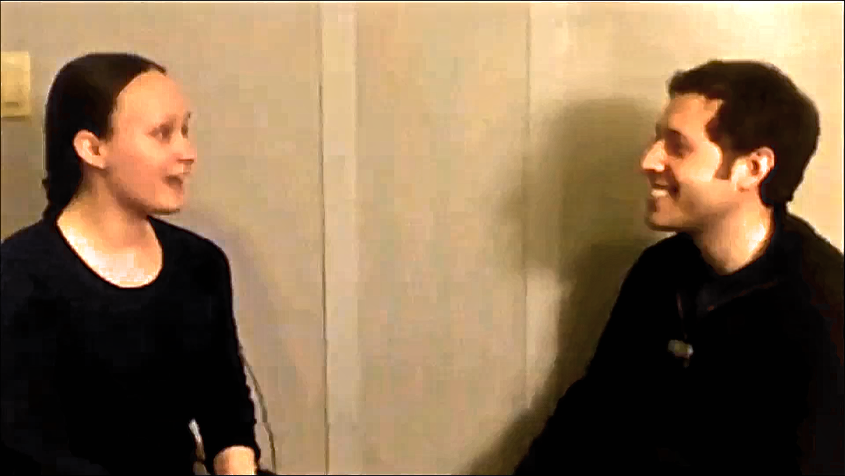
\includegraphics[width=0.6\textwidth]{figures/FIG-FL-stim.png}
\end{center}
\caption{Example frame from a conversation video used in Experiment 1.} 
\label{fig:speakers}
\end{figure}

\subsubsection{Materials}

\textit{Video recordings}. We recorded pairs of talkers while they conversed in a sound-attenuated booth (see sample frame in Figure \ref{fig:speakers}). Each talker was a native speaker of the language being recorded, and each talker pair was male-female. Using a Marantz PMD 660 solid state field recorder, we captured audio from two lapel microphones, one attached to each participant, while simultaneously recording video from the built-in camera of a MacBook laptop computer. The talkers were volunteers and were acquainted with their recording partner ahead of time. 

Each recording session began with a 20-minute warm-up period of spontaneous conversation during which the pair talked for five minutes on four topics (favorite foods, entertainment, hometown layout, and pets). Then we asked talkers to choose a new topic---one relevant to young children (e.g., riding a bike, eating breakfast)---and to improvise a dialogue on that topic. We asked them to speak as if they were on a children's television show in order to elicit child-directed speech toward each other. We recorded until the talkers achieved at least 30 seconds of uninterrupted discourse with enthusiastic, child-directed speech. Most talker pairs took less than five minutes to complete the task, usually by agreeing on a rough script at the start. We encouraged talkers to ask at least a few questions to each other during the improvisation. The resulting conversations were therefore not entirely spontaneous, but were as close as possible while still remaining child-oriented in topic, prosodic pattern, and lexicosyntactic construction.\footnote{All of the non-English talkers were fluent in English as a second language, and some fluently spoke a third or more language. We chose male-female pairs as a natural way of creating contrast between the two talker voices.}

%% PART UNFINISHED: link for example video

After recording, we combined the audio and video files by hand, and cropped each recording to the 30-second interval with the most turn activity. Because we recorded the conversations in stereo, the male and female voices came out of separate speakers during video playback. This gave each voice in the videos a localized source (from the left or right loudspeaker). We coded each turn transition in the videos for language condition (English vs. non-English), inter-turn gap duration (in milliseconds), and speech act (question vs. non-question). The non-English stimuli were coded for speech act from a monolingual English-speaker's perspective, i.e., which turns ``sound like'' questions, and which don't: we asked five native American English speakers to listen to the audio signal for each turn and judge whether it sounded like a question. We then coded turns with at least 80\% ``yes'' responses as questions.

Because the conversational stimuli were recorded semi-spontaneously, the duration of turn transitions and the number of speaker transitions in each video was variable. We measured the duration of each turn transition from the audio recording associated with each video. We excluded turn transitions longer than 550 msec and shorter than 90 msec, including overlapped transitions, from analysis.\footnote{Overlap occurs when a responder begins a new turn before the current turn is finished. When overlap occurs, observers cannot switch their gaze in anticipation of the response because the response began earlier than expected; participants expect conversations to proceed with ``one speaker at a time'' \citep{sacks1974}. As such, they would still be fixated on the prior speaker when the overlap started, and then would have to switch their gaze \textit{reactively} to the responder.} This left approximately equal numbers of turn transitions available for analysis in the English (N$=$20) and non-English (N$=$16) videos. On average, the inter-turn gaps for English videos (mean$=$318, median$=$302, stdv$=$112 msec) were slightly longer than for non-English videos (mean$=$286, median$=$251, stdv$=$122 msec). The longer gaps in the English videos could give them a slight advantage: Our definition of an ``anticipatory gaze shift'' includes shifts that are initiated during the gap between turns (Figure \ref{fig:criterion}), so participants had slightly more time to make anticipatory shifts in the English videos.

Questions made up exactly half of the turn transitions in the English (N$=$10) and non-English (N$=$8) videos. In the English videos, inter-turn gaps were slightly shorter for questions (mean$=$310, median$=$293, stdev$=$112 msec) than non-questions (mean$=$325, median$=$315, stdv$=$118 msec). Non-English videos did not show a large difference in transition time for questions (mean$=$270, median$=$257, stdv$=$116 msec) and non-questions (mean$=$302, median$=$252, stdv$=$134 msec).

\subsubsection{Procedure} 
Participants sat in front of an SMI 120Hz corneal reflection eye-tracker mounted beneath a large flatscreen display. The display and eye-tracker were secured to a table with an ergonomic arm that allowed the experimenter to position the whole apparatus at a comfortable height, approximately 60 cm from the viewer. We placed stereo speakers on the table, to the left and right of the display. 

Before the experiment started, we warned adult participants that they would see videos in several languages and that, though they weren't expected to understand the content of non-English videos, we \textit{would} ask them to answer general, non-language-based questions about the conversations. Then after each video we asked participants one of the following randomly-assigned questions: ``Which speaker talked more?'', ``Which speaker asked the most questions?'', ``Which speaker seemed more friendly?'', and ``Did the speakers' level of enthusiasm shift during the conversation?'' We also asked if the participants could understand any of what was said after each video. The participants responded verbally while an experimenter noted their responses.

Children were less inclined to simply sit and watch videos of conversation in languages they didn't speak, so we used a different procedure to keep them engaged: The experimenter started each session by asking the child about what languages he or she could speak, and about what other languages he or she had heard of. Then the experimenter expressed her own enthusiasm for learning about new languages, and invited the child to watch a video about ``new and different languages'' together. If the child agreed to watch, the experimenter and the child sat together in front of the display, with the child centered in front of the tracker and the experimenter off to the side. Each conversation video was preceded and followed by a 15--30 second attention-getting filler video (e.g., running puppies, singing muppets, flying bugs). If the child began to look bored, the experimenter would talk during the fillers, either commenting on the previous conversation (``That was a neat language!'') or giving the language name for the next conversation (``This next one is called Hebrew. Let's see what it's like.'') The experimenter's comments reinforced the video-watching as a joint task.

All participants (child and adult) completed a five-point calibration routine before the first video started. We used a dancing Elmo for the children's calibration image. During the experiment, participants watched all six 30-second conversation videos. The first and last conversations were in American English and the intervening conversations were Hebrew, Japanese, German, and Korean. The presentation order of the non-English videos was shuffled into four lists, which participants were assigned to randomly. The entire experiment, including instructions, took 10--15 minutes.

\subsubsection{Data preparation and coding}
\label{sec:algorithm}

To determine whether participants predicted upcoming turn transitions, we needed to define a set of criteria for what counted as an anticipatory gaze shift. Prior work using similar experimental procedures has found that adults and children make anticipatory gaze shifts to upcoming talkers within a wide time frame; the earliest shifts occur before the end of the prior turn, and the latest occur after the onset of the response turn, with most shifts occurring in the inter-turn gap (Keitel et al., 2013; Hirvenkari, 2013; Tice and Henetz, \citeyear{TiceHenetz11}). Following prior work, we measured how often our participants shifted their gaze from the prior to the upcoming speaker \textit{before} the shift in gaze could have been initiated in reaction to the onset of the speaker's response. In doing so, we assumed that it takes participants 200 msec to plan an eye movement, following standards from adult anticipatory processing studies \citep[e.g., ][]{kamide2003}.

We checked each participant's gaze at each turn transition for three characteristics (Figure \ref{fig:criterion}): (1) That the participant fixated on the prior speaker for at least 100 msec at the end of the prior turn, (2) that sometime thereafter the participant switched to fixate on the upcoming speaker for at least 100 ms, and (3) that the switch in gaze was initiated within the first 200 msec of the response turn, or earlier. These criteria guarantee that we only counted gaze shifts when: (1) Participants were tracking the previous speaker, (2) switched their gaze to track the upcoming speaker, and (3) did so before they could have simply reacted to the onset of speech in the response. Under this assumption, a gaze shift that was initiated within the first 200 msec of the response (or earlier) was planned \textit{before} the child could react to the onset of speech itself. 

As mentioned, most anticipatory switches happen in the inter-turn gap, but we also allowed anticipatory gaze switches that occurred in the final syllables of the prior turn. Early switches are consistent with the distribution of responses in explicit turn-boundary prediction tasks. For example, in a button press task, adult participants anticipate turn ends approximately 200 msec in advance of the turn's end, and anticipatory responses to pitch-flattened stimuli come even earlier \citep{de-ruiter2006}. We therefore allowed switches to occur as early as 200 msec before the end of the prior turn. For very early and very late switches, our requirement for 100 msec of fixation on each speaker would sometimes extend outside of the transition window boundaries (200 msec before and after the inter-turn gap). The maximally available fixation window was 100 msec before and after the earliest and latest possible switch point (300 msec before and after the inter-turn gap). We did not count switches made during the fixation window as anticipatory. We \textit{did} count switches made during the inter-turn gap. The period of time from the beginning of the possible fixation window on the prior speaker to the end of the possible fixation window on the responder was our total analysis window (300 msec $+$ the inter-turn gap $+$ 300 msec).

\begin{figure}[t]
\begin{center}
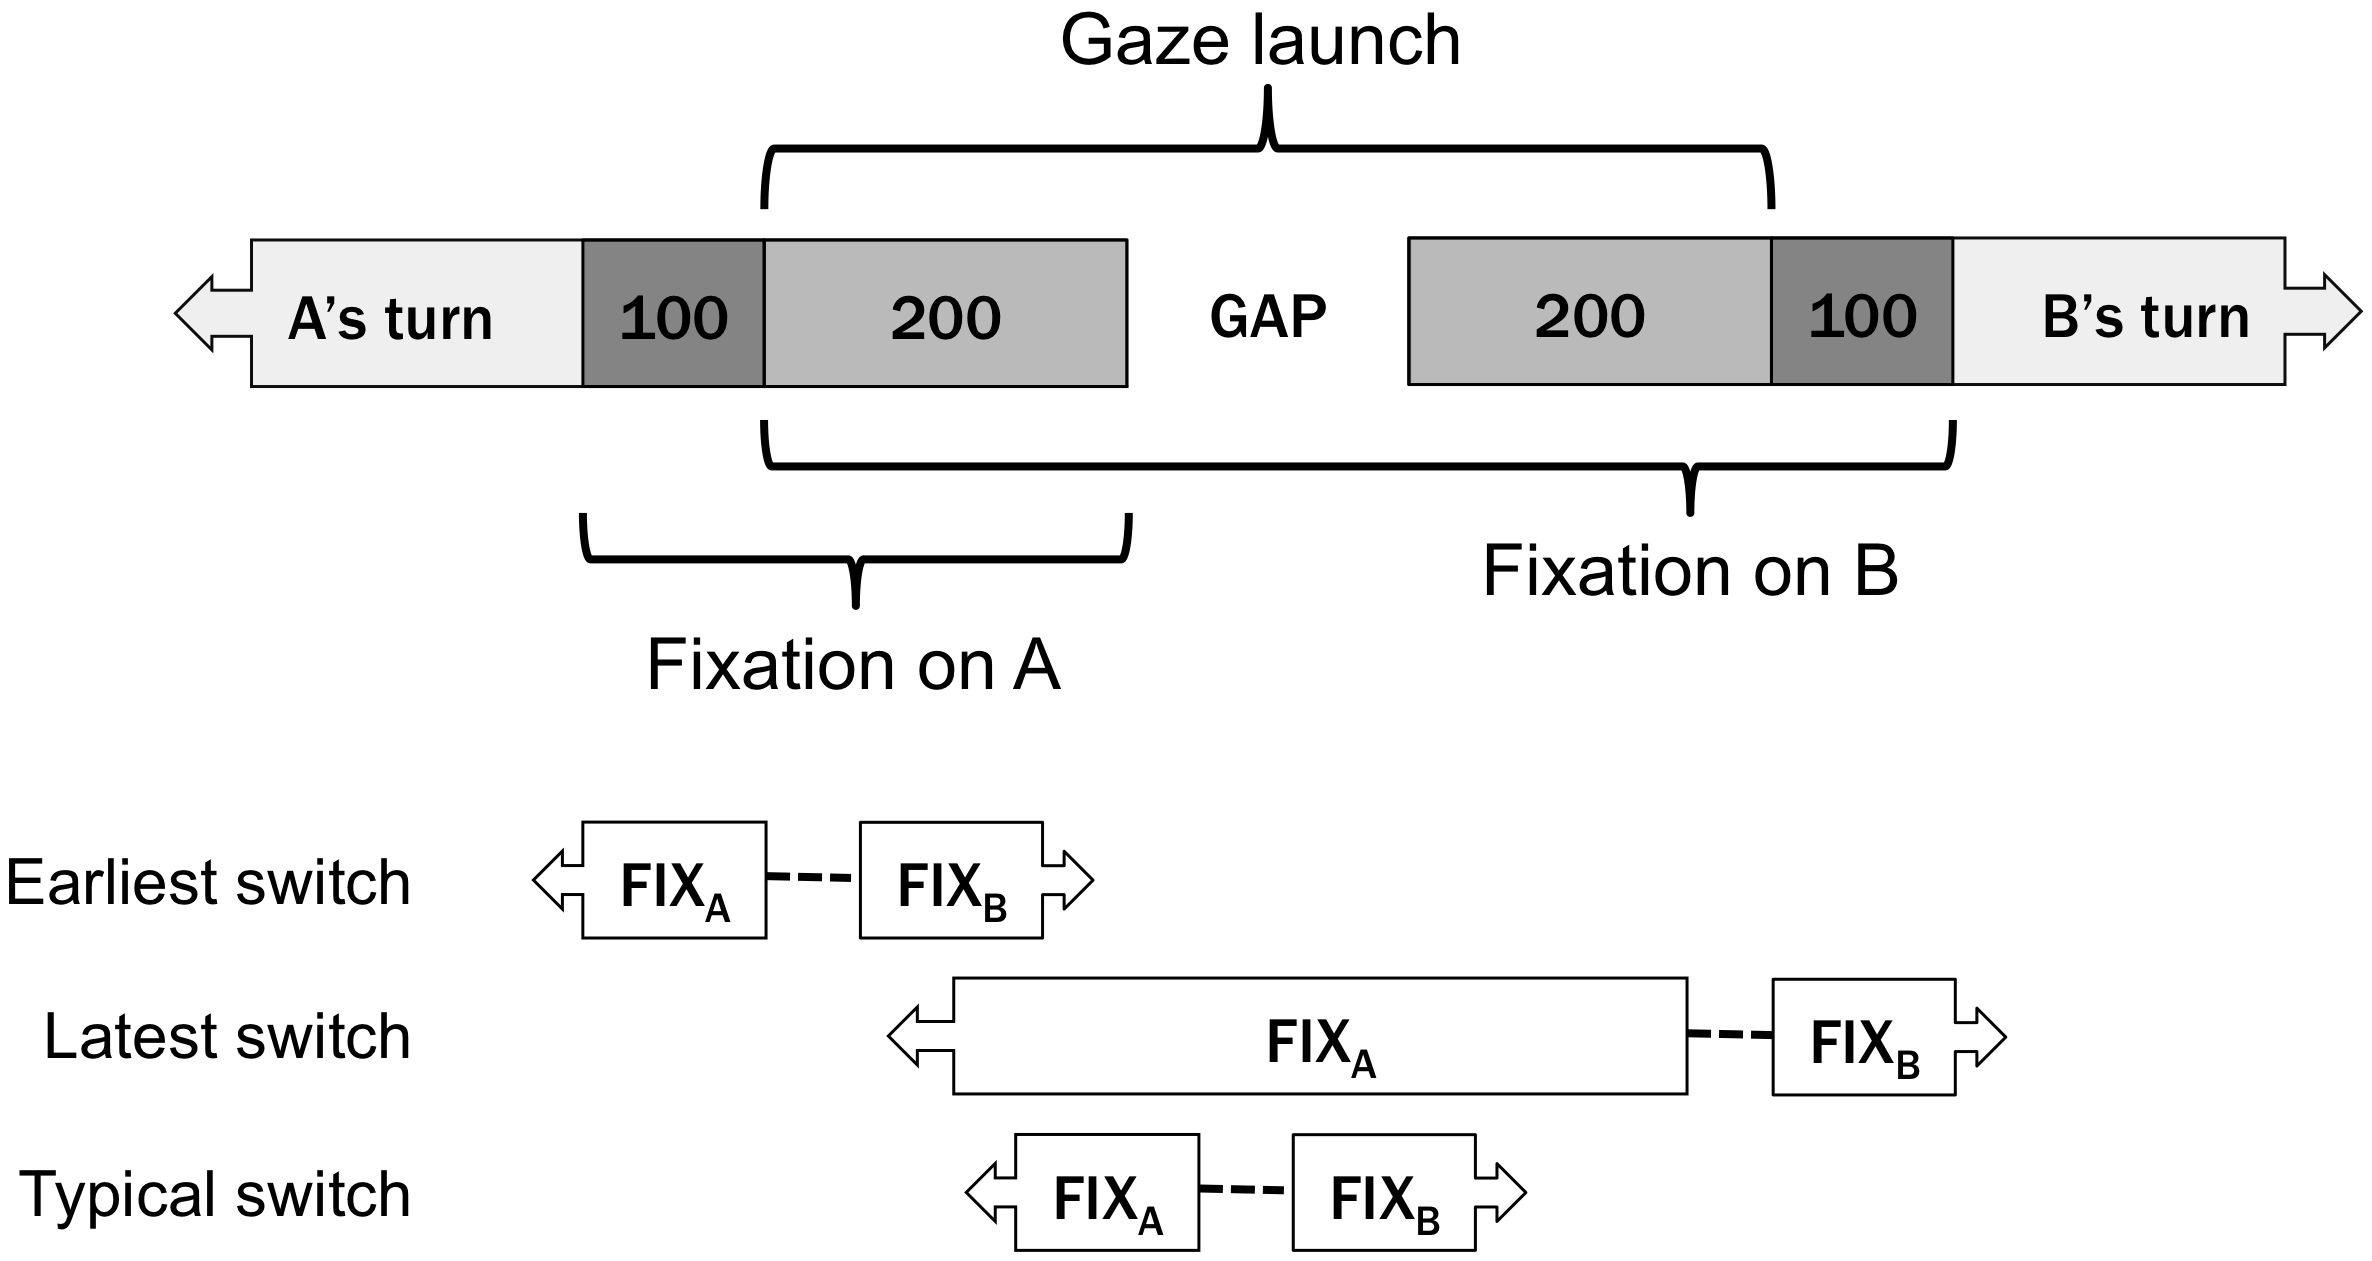
\includegraphics[width=0.7\textwidth]{figures/FIG-AnticipCriteria.png}
\end{center}
\caption{Schematic summary of criteria for anticipatory gaze shifts from speaker A to speaker B during a turn transition.} 
\label{fig:criterion}
\end{figure}

\paragraph{Predictions}
We expected participants to show greater anticipation in the English videos than in the non-English videos because of their increased access to linguistic information in English. We also predicted that anticipation would be greater following questions compared to non-questions; questions have early cues to upcoming turn transition (e.g., \textit{wh-} words, subject-auxiliary inversion), and also make a next response immediately relevant. Our third prediction was that anticipatory looks would increase with development, along with children's increased linguistic competence.

\subsection{Results}
\label{sec:results1}

Participants looked at the screen most of the time during video playback (81\% and 91\% on average for children and adults, respectively). They primarily kept their eyes on the person who was currently speaking in both English and non-English videos: They gazed at the current speaker between 38\% and 63\% of the time, looking back at the addressee between 15\% and 20\% of the time (Table \ref{tab:e1_look}). Even three-year-olds looked more at the current speaker than anything else, whether the videos were in a language they could understand or not. Children looked at the current speaker less than adults did during the non-English videos. Despite this, their looks to the addressee did not increase substantially in the non-English videos, indicating that their looks away were probably related to boredom rather than confusion about ongoing turn structure. Overall, participants' pattern of gaze to current speakers demonstrated that they performed basic turn tracking during the videos, regardless of language.

\begin{table}[t]
\begin{center}
  \begin{tabular}{llcccc}
    \hline
    Age group & Condition & Speaker & Addressee & Other onscreen & Offscreen\\ 
    \hline
    3 & English & 0.61 & 0.16 & 0.14 & 0.08 \\ 
    4 & English & 0.60 & 0.15 & 0.11 & 0.13 \\ 
    5 & English & 0.57 & 0.15 & 0.16 & 0.12 \\ 
    Adult & English & 0.63 & 0.16 & 0.16 & 0.05 \\ 
    3 & Non-English & 0.38 & 0.17 & 0.20 & 0.25 \\ 
    4 & Non-English & 0.43 & 0.19 & 0.21 & 0.18 \\ 
    5 & Non-English & 0.40 & 0.16 & 0.26 & 0.18 \\ 
    Adult & Non-English & 0.58 & 0.20 & 0.16 & 0.07 \\ 
%   Overall & & 0.49 & 0.17 & 0.18 & 0.16 \\
    \hline
  \end{tabular}
\end{center}
  \caption{Average proportion of gaze to the current speaker and addressee during periods of talk.}
\label{tab:e1_look}
\end{table}

\begin{table}[h!]
\begin{center}
  \begin{tabular}{lcccl}
  \textbf{\textit{Children}} &&&& \\
    \hline
                   & Estimate & Std. Error & z value & Pr($>$$|$z$|$)    \\
    \hline
    (Intercept)   &      -0.96146 &   0.84901 & -1.132 & 0.257446 \\    
    Age             &    -0.18268 &   0.17507 & -1.043 & 0.296725   \\  
    LgCond$=$\textit{non-English} &          -3.29347 &   0.96045 & -3.429 & 0.000606 *** \\
    Type$=$\textit{non-Question}          &     -1.10129 &   0.86494 & -1.273 & 0.202925     \\
    Duration      &       3.40169 &   1.22826 &  2.770 & 0.005614  **\\
    Age*LgCond$=$\textit{non-English} &       0.52065 &   0.21190 &  2.457 & 0.014008 ** \\  
    Age*TypeS$=$\textit{non-Question}          & -0.01628 &   0.19437 & -0.084 & 0.933232     \\
    LgCond$=$\textit{non-English}* &     2.68166 &   1.35016 &  1.986 & 0.047013 * \\
    Type$=$\textit{non-Question} &&&& \\
    Age*LgCond$=$\textit{non-English}* & -0.45632 &   0.30163 & -1.513 & 0.130315  \\
    Type$=$\textit{non-Question} &&&& \\
    \hline
  &&&& \\
  \textbf{\textit{Adults}} &&&& \\
    \hline
                       &  Estimate & Std. Error & z value & Pr($>$$|$z$|$) \\    
    \hline
    (Intercept)       &        -0.1966 &    0.6942 & -0.283 & 0.776988     \\
    LgCond$=$\textit{non-English}    &             -0.8812 &    0.9602 & -0.918 & 0.358754   \\  
    Type$=$\textit{non-Question}             &        -4.4953 &    1.3139 & -3.421 & 0.000623 *** \\
    Duration          &        -1.1227 &    1.9880 & -0.565 & 0.572238     \\
    LgCond$=$\textit{non-English}* &           3.2972 &    1.6101 &  2.048 & 0.040581 * \\ 
    Type$=$\textit{non-Question} &&&& \\
    LgCond$=$\textit{non-English}* &        1.3626 &    3.0077 &  0.453 & 0.650527     \\
    Duration &&&& \\
    Type$=$\textit{non-Question}*          &  10.5107 &    3.3459 &  3.141 & 0.001682  ** \\
    Duration &&&& \\
    LgCond$=$\textit{non-English}* & -6.3156 &    4.4926 & -1.406 & 0.159790 \\    
    Type$=$\textit{non-Question}* &&&& \\
    Duration &&&& \\
    \hline
  \end{tabular}
\end{center}
  \caption{Model output for children and adults' anticipatory gaze switches.}
\label{tab:E1-models}
\end{table}

\subsubsection{Statistical models}
\label{sec:models1}

We identified anticipatory gaze switches for all 36 usable turn transitions, based on the criteria outlined in Section \ref{sec:algorithm}, and analyzed them for effects of language, transition type, and age with two mixed-effects logistic regressions \citep{lme4, R}. We built one model each for children and adults. We modeled children and adults separately because effects of age are only pertinent to the children's data. The child model included condition (English vs. non-English)\footnote{Because each non-English language was represented by a single stimulus, we cannot treat individual languages as factors. Gaze behavior might be best for non-native languages that have the most structural overlap with participants' native language: English speakers can make predictions about the strength of upcoming Swedish prosodic boundaries nearly as well as Swedish speakers do, but Chinese speakers are at a disadvantage in the same task \citep{carlson2005}. We would need multiple items from each of the languages to check for similarity effects of specific linguistic features.}, transition type (question vs. non-question), age (3, 4, 5), and duration of the inter-turn gap (seconds, e.g., 0.441) as predictors, with full interactions between condition, transition type, and age.  We included the duration of the inter-turn gap as a predictor since longer gaps also provide more opportunities to make anticipatory switches (Figure \ref{fig:criterion}). We additionally included random effects of item (turn transition) and participant, with random slopes of condition, transition type, and their interaction for participants \citep{barr2013}.\footnote{The models we report are all qualitatively unchanged by the exclusion of their random slopes. We have left the random slopes in because of minor participant-level variation in the predictors modeled.} The adult model included condition, transition type, duration, and their interactions as predictors with participant and item included as random effects and random slopes of condition, transition type, and their interaction for participant.

Children's anticipatory gaze switches showed effects of language condition (\textit{$\beta$}=-3.29, \textit{SE}=0.961, \textit{t}=-3.43, \textit{p}$<$.001) and gap duration (\textit{$\beta$}=3.4, \textit{SE}=1.229, \textit{t}=2.77, \textit{p}$<$.01) with additional effects of an age-by-language condition interaction (\textit{$\beta$}=0.52, \textit{SE}=0.212, \textit{t}=2.46, \textit{p}$<$.05) and a language condition-by-transition type interaction (\textit{$\beta$}=2.68, \textit{SE}=1.35, \textit{t}=1.99, \textit{p}$<$.05). There were no significant effects of age or transition type alone (\textit{$\beta$}=-0.18, \textit{SE}=0.175, \textit{t}=-1.04, \textit{p}$=$.3 and \textit{$\beta$}=-1.10, \textit{SE}=0.865, \textit{t}=-1.27, \textit{p}$=$.2, respectively). 

Adults' anticipatory gaze switches shows an effect of transition type (\textit{$\beta$}=-4.5, \textit{SE}=1.314, \textit{t}=-3.42, \textit{p}$<$.001) and significant interactions between language condition and transition type (\textit{$\beta$}=3.3, \textit{SE}=1.61, \textit{t}=2.05, \textit{p}$<$.05) and transition type and gap duration (\textit{$\beta$}=10.51, \textit{SE}=3.346, \textit{t}=3.141, \textit{p}$<$.01).

\subsubsection{Random baseline comparison}
\label{sec:randbaseline1}

We estimated the probability that these patterns were the result of random looking by running the same regression models on participants' real eye-tracking data, only this time calculating their anticipatory gaze switches with respect to randomly permuted turn transition windows. This process involved: (1) randomizing the order and temporal placement of the analysis windows within each stimulus (Figure \ref{fig:shuffling}; ``analysis window'' is defined in Figure \ref{fig:criterion}), thereby randomly redistributing the analysis windows across the eye-tracking signal, (2) re-running each participant's eye tracking data through switch identification (described in \ref{sec:algorithm}), this time using the randomly permuted analysis windows, and (3) modeling the anticipatory gazes from the randomly permuted data with the same statistical models we used for the original data (Section \ref{sec:models1}; Table \ref{tab:E1-models}). Importantly, although the onset time of each transition was shuffled within the eye-tracking signal, the other intrinsic properties of each turn transition (e.g., prior speaker identity, transition type, gap duration, language condition, etc.) stayed constant across each random permutation. 

\begin{figure}[ht!]
\begin{center}
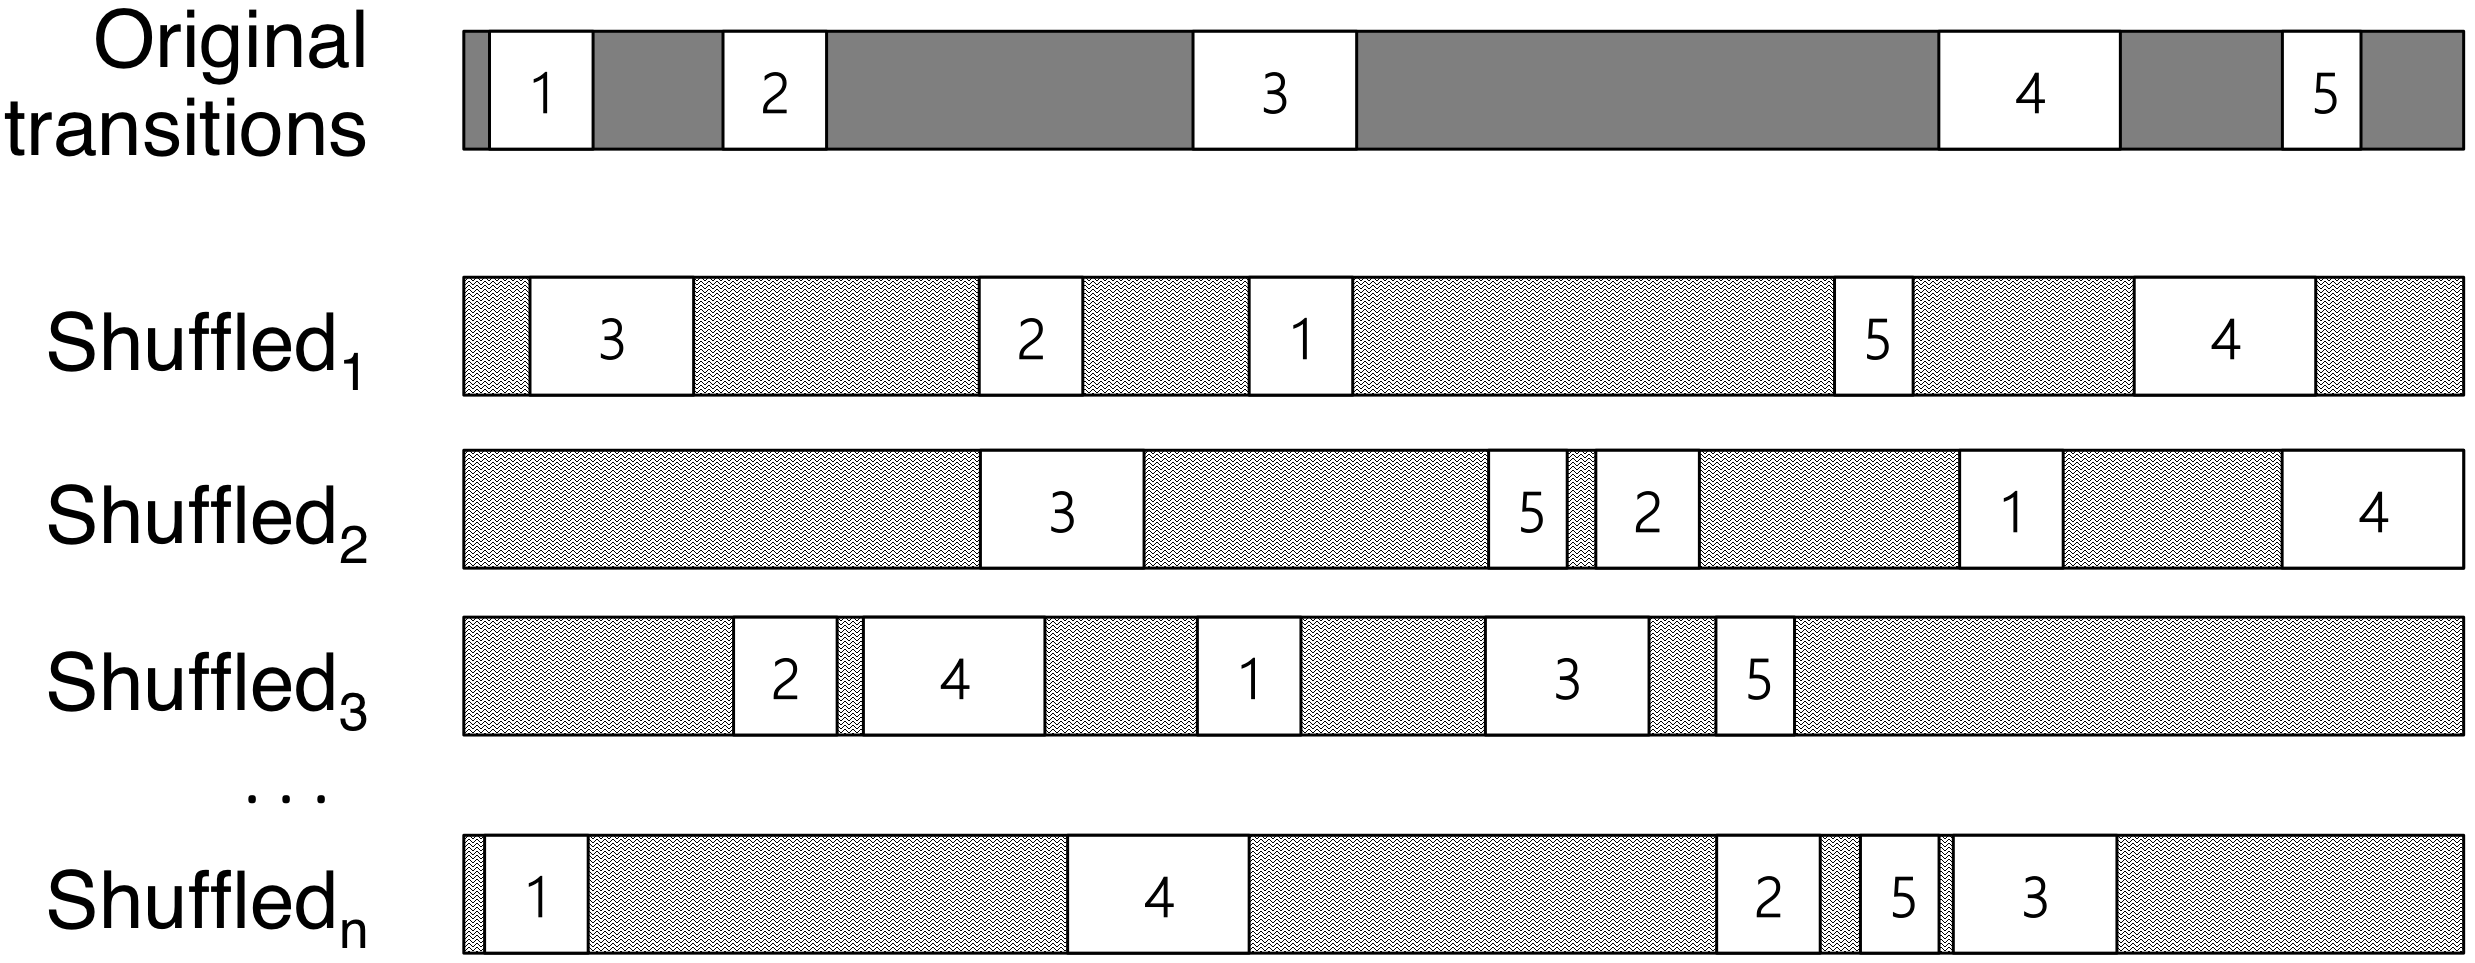
\includegraphics[width=0.8\textwidth]{figures/FIG-ShuffledWindows.png}
\end{center}
\caption{Example of shuffling for five turn transition analysis windows. The windows were $\pm$300 msec around the inter-turn gap.} 
\label{fig:shuffling}
\end{figure}

This procedure effectively de-links participants' gaze data from the turn structure in the original stimulus, thereby allowing us to compare turn-related (original) and non-turn-related (randomly permuted) looking behavior using the same eye movements. The resulting anticipatory gazes from the randomly permuted analysis windows represent an average anticipatory gaze rate over all possible starting points: a random baseline. By running the real and randomly permuted data sets through identical statistical models, we can also estimate how likely it is that predictor effects in the original data (e.g., the effect of language condition; Table \ref{tab:E1-models}) arose from random looking.

We completed this baseline procedure on 5,000 random permutations of the original turn transition analysis windows and compared the \textit{t}-values from each predictor in the original models (Table \ref{tab:E1-models}) to the distribution of \textit{t}-values for each predictor in the 5,000 models of the randomly permuted datasets.\footnote{We report \textit{t}-values rather than beta estimates because the standard errors in the randomly permuted data models were much higher than for the original data. For those interested, plots of the beta and standard error distributions are available in the Appendix.} We could then test whether significant effects from the original statistical models differed from the random baseline by calculating the proportion of random data \textit{t}-values exceeded by the original \textit{t}-value for each predictor, using the absolute value of all \textit{t}-values for a two-tailed test. For example, children's original ``language condition'' \textit{t}-value was $|$3.429$|$, which is greater than 99.9\% of all $|$\textit{t}-value$|$ estimates from the randomly-permuted data models (i.e., \textit{p} $=$ .001). This leads us to conclude that that the effect of language condition in the original model was highly unlikely to be the result of random gaze shifting.

\begin{figure}[h!]
  \centering
  \subfloat[Children]{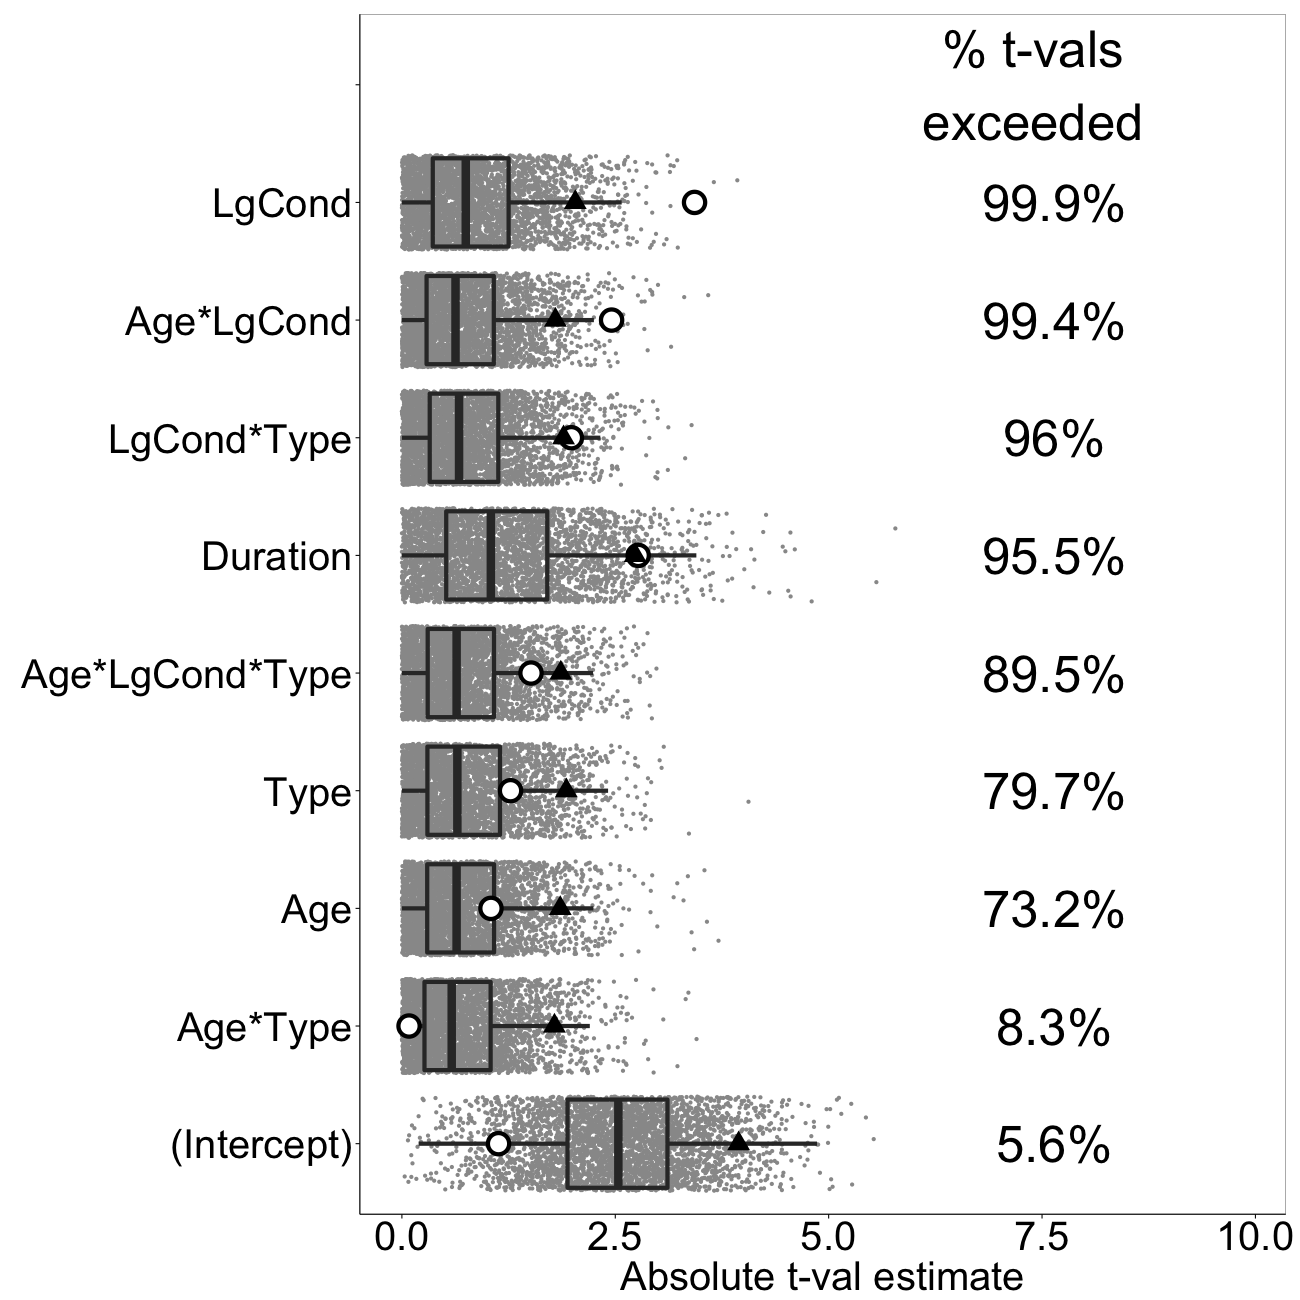
\includegraphics[width=0.49\textwidth]{figures/E1-chi-randrun-t-vals-absolute.png}\label{fig:E1-ChiTs}}
  \hfill
  \subfloat[Adults]{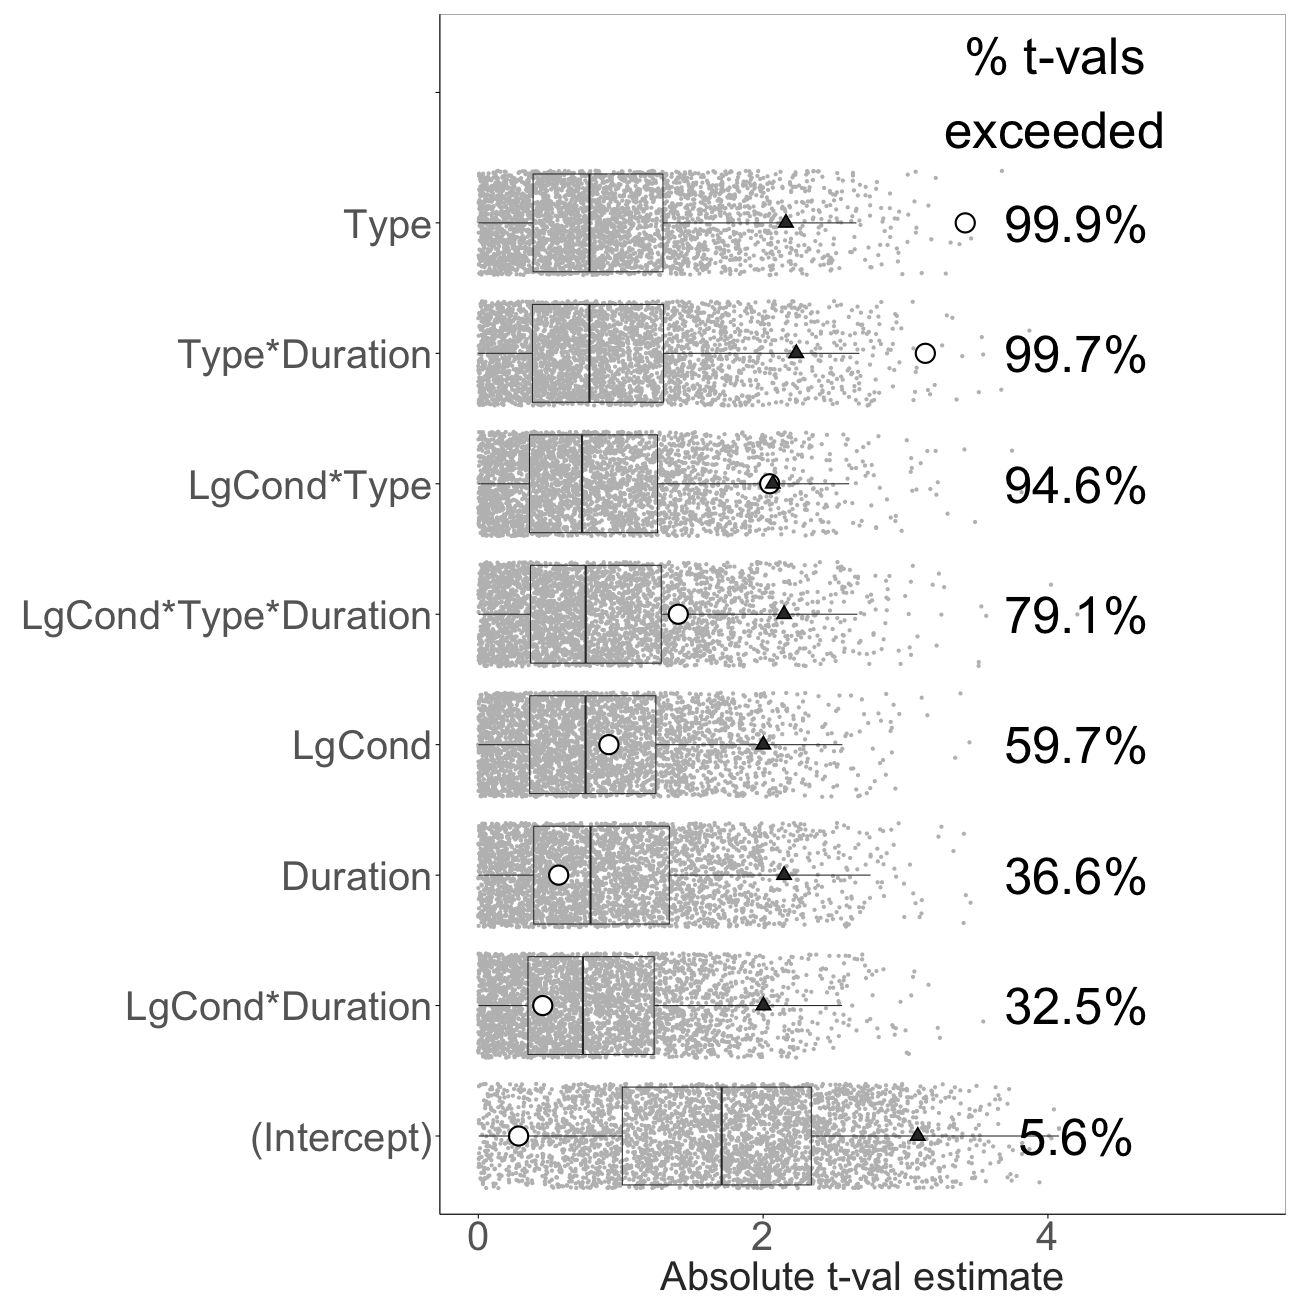
\includegraphics[width=0.49\textwidth]{figures/E1-adu-randrun-t-vals-absolute.png}\label{fig:E1-AduTs}}
  \caption{Random-permutation and original $|$\textit{t}-values$|$ for predictors of children and adults' anticipatory gaze rates. Gray dots $=$ random model estimates, White dots $=$ original model estimates, Triangles $=$ 95th percentile for each \textit{t}-value distribution.}
\end{figure}

% PART UNFINISHED (potentially)
% We excluded the output of random-permutation models that did not converge to remove unreliable model results from our percentile calculations below (XX\% and XX\% of models for children and adults, respectively). 

Our baseline analyses revealed that none of the significant predictors from models of the original, turn-related data can be explained by random looking. The children's data showed strong evidence of differentiation from the randomly permuted data for all four significant effects in the original model (Table \ref{tab:E1-models}: Children):  the original \textit{t}-values for language condition, gap duration, the age-language condition interaction, and the language condition-transition type interaction were all greater than 95\% of \textit{t}-values for the randomly permuted data (99.9\%, 95.5\%, 99.4\%, and 96\%, respectively; Figure \ref{fig:E1-ChiTs}). Similarly, the adults' data showed significant differentiation from the randomly permuted data for two of the three originally significant predictors---transition type and the transition type-gap duration interaction (greater than 99.9\% and 99.7\% of random \textit{t}-values, respectively)---with marginal differentiation for the interaction of language condition and transition type (greater than 94.7\% of random \textit{t}-values; Figure \ref{fig:E1-AduTs}). The effects of language condition and transition type for the real and randomly permuted data can also be observed in Figure \ref{fig:E1-randvsreal}.

\begin{figure}[h]
\begin{center}
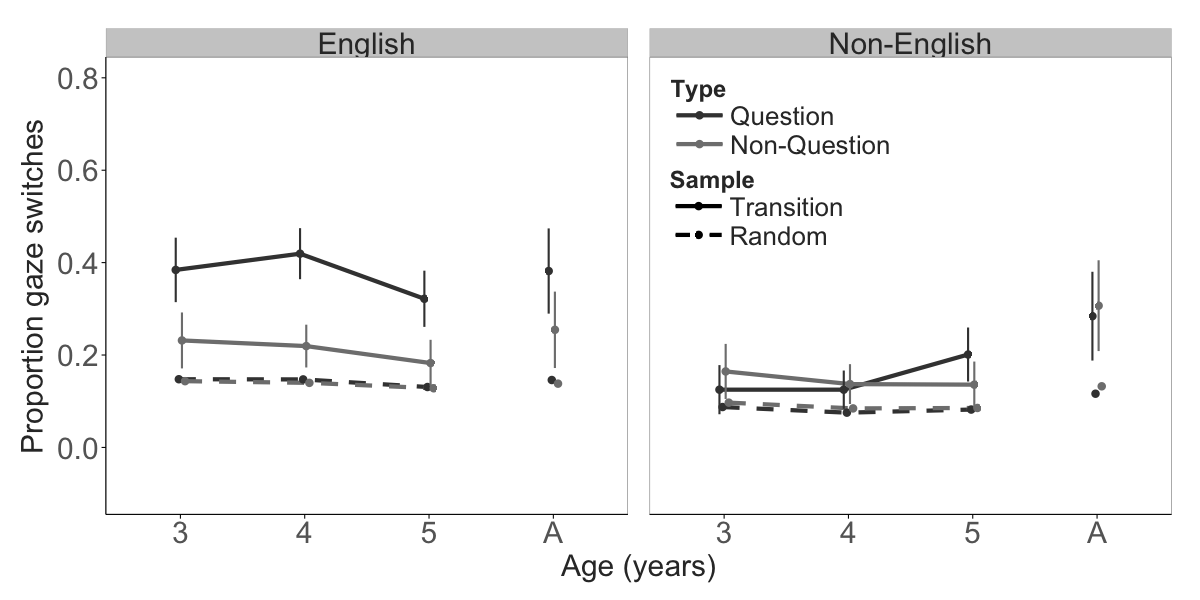
\includegraphics[width=0.8\textwidth]{figures/E1-samples-by-lang-groups-trans-types.png}
\end{center}
\caption{Anticipatory gaze rates across language condition and transition type for the real (red and blue) and randomly permuted (gray) data. Vertical bars represent the standard error.} 
\label{fig:E1-randvsreal}
\end{figure}

\begin{figure}[h!]
\begin{center}
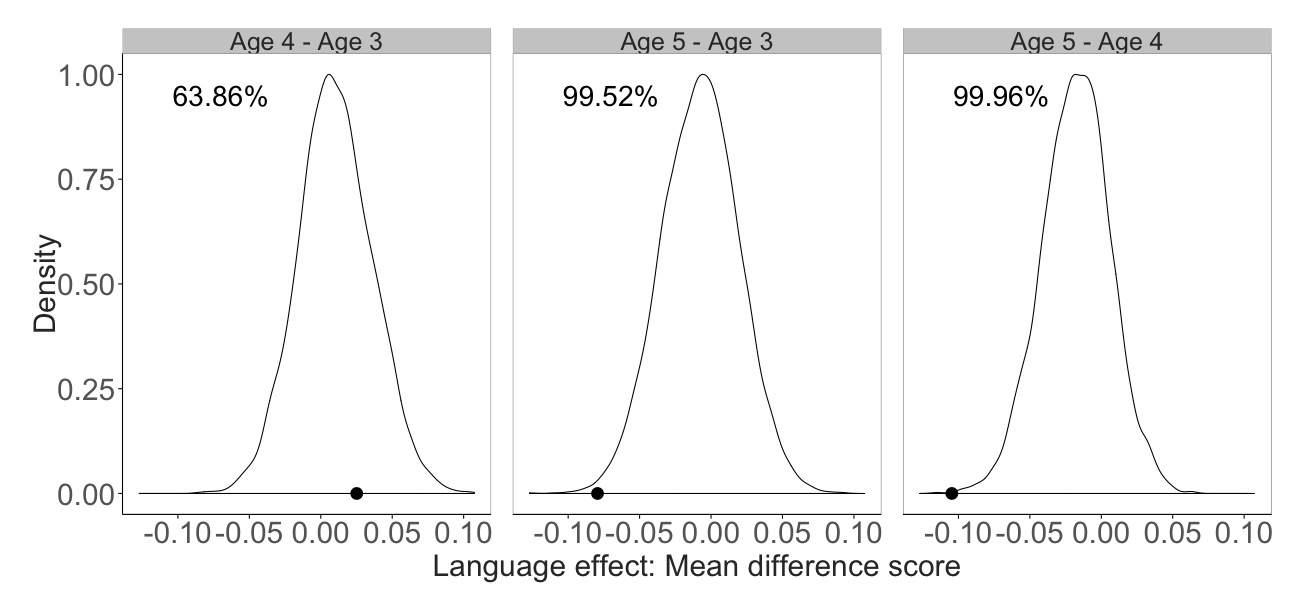
\includegraphics[width=0.8\textwidth]{figures/E1-child-randvsreal-ttest-agebylg.png}
\end{center}
\caption{Pairwise comparisons of the language condition effect across ages for the original data (black dots) and the 5,000 randomly permuted datasets (distribution).} 
\label{fig:E1-lgageinteraction}
\end{figure}

\paragraph{Developmental effects}
The model of the children's data revealed a significant interaction of age and language condition (Table \ref{tab:E1-models}) that was highly unlikely to have derived from random looking (Figure \ref{fig:E1-randvsreal}). To further explore this effect, we compared the average effect of language condition across all ages: we extracted the average difference score for the two language conditions (English minus non-English) for each subject, computing an overall average for each random permutation of the data. For each random permutation, we then made pairwise comparisons of the average difference scores across ages. Figure \ref{fig:E1-lgageinteraction} plots the real-data difference scores against the random-data difference score distribution for each pairwise age comparison, showing that 3- and 4-year olds were affected equally by language condition, but that 5-year-olds affected less than both 3- and 4-year-olds (with 99.52\% and 99.96\% of difference scores greater than the randomly permuted data, respectively, i.e., differences of \textit{p} $<$ .01 and \textit{p} $<$ .001).

\subsection{Discussion}
\label{sec:discussion1}

Children and adults spontaneously tracked the turn structure of the conversations, making anticipatory gaze switches at an above-chance rate across all ages and conditions (Table \ref{tab:e1_look}; Figure \ref{fig:E1-randvsreal}). Children's anticipatory gaze rates were affected by language condition, transition type, age, and gap duration (Table \ref{tab:E1-models}), none of which could be explained by a baseline of random gaze switching (Figure \ref{fig:E1-ChiTs}).

Language condition (English vs. non-English) affected children's anticipations in two ways (Table \ref{tab:E1-models};  Figure \ref{fig:E1-randvsreal}). First, children made more anticipatory switches overall in English videos, compared to non-English videos. This effect suggests that lexical access is important for children's ability to anticipate upcoming turn structure; children had no lexical access to the speech in the non-English videos, though they did have access to (non-native) prosodic cues and non-verbal behavior, consistent with prior work on turn-end prediction in adults (\citealp{de-ruiter2006}; \citealp{magyari2012}) and children \citep{keitel2013}. Second, children systematically made more anticipatory switches after hearing a question compared to a non-question, but only in the English condition, suggesting that, when children have access to lexical cues, they are more likely to make an anticipatory gaze switch if they can expect an immediate response from the addressee. If so, then children's attention to lexical cues for turn taking may primarily be in monitoring the signal for cues to questionhood (e.g., subject-auxiliary inversion, \textit{wh}-words, etc.).

Children's anticipatory gaze switches were also affected by their age, but only in the non-English videos: 3- and 4-year-olds made many more anticipatory switches when watching videos in English compared to non-English, but this effect of language condition had attenuated significantly by age 5 (Table \ref{tab:E1-models};  Figure \ref{fig:E1-randvsreal}; Figure \ref{fig:E1-lgageinteraction}). This interaction suggests that the 5-year-olds were able to leverage anticipatory cues in the non-English videos in a way that 3- and 4-year-olds could not, possibly by shifting more attention to the non-native prosodic or non-verbal cues. Prior work on children's turn-structure anticipation proposed that children's turn-end predictions rely primarily on lexicosyntactic structure (and not, e.g., prosody) as they get older \citep{keitel2013}. The current results suggest more flexibility in children's predictions; when they do not have access to lexical information, older children are likely to find alternative cues to turn taking behavior.

Finally, children showed an effect of gap duration (Table \ref{tab:E1-models}). This effect is straightforward: longer gaps resulted in longer analysis windows, yielding more time for children to make an anticipatory gaze.

Adults' anticipatory gaze rates were also affected by transition type, language condition, and gap duration (Table \ref{tab:E1-models}), none of which could be easily explained by a baseline of random gaze switching (Figure \ref{fig:E1-AduTs}). Like children, adults made more anticipatory switches after hearing questions compared to non-questions, suggesting that anticipation mattered more to them when an immediate response was expected. Also like children, the advantage for questions was driven by lexical access such that adults must have relied on lexicosyntactic cues to questionhood in picking out turns that potentially require an immediate response, though this effect was only marginally divergent from the distribution of randomly permuted data (\textit{p} $=$ .053; Figure \ref{fig:E1-AduTs}). Finally, adults' anticipation rates were also affected by gap duration, but more so for questions than non-questions (Table \ref{tab:E1-models}). This interaction suggests that adults were less likely overall to make anticipatory switches at non-questions (as is evident for adults and children in Figure \ref{fig:E1-randvsreal}), and so did not benefit from extra time to do so compared to long gaps for questions.

\subsubsection{Summary}
\label{sec:summary1}

Children and adults' predictions alike were benefited by access to lexical information (English) and speech act status (questionhood), suggesting that linguistic cues, particularly lexical ones, facilitate their spontaneous predictions about upcoming turn structure through the identification of turns with immediate responses. Children's anticipatory gaze rates for questions and non-questions in English was stable across ages and comparable to adult behavior (Figure \ref{fig:E1-randvsreal}), suggesting that they can identify questions in native stimuli with adult-like competence by age three. Although participants' ability to recognize questions was facilitated by lexical access (i.e., English vs. non-English), the prosody in the non-English videos was non-native, and so the experimental design can not conclusively show which linguistic cues children relied on in the English videos to identify question turns. Relatedly, though lexical access clearly facilitated participants' anticipatory gaze rate, it was not necessary for participants---especially adults---in order to exceed chance switching rates (Figure \ref{fig:E1-randvsreal}), suggesting that participants use non-lexical cues (e.g., prosody, non-verbal behavior) to make anticipatory eye movements at least some of the time.

Interestingly, adults and children both were strongly affected by transition type, in that they made more anticipatory switches after hearing questions, compared to non-questions. Even in the English videos, when participants had full access to linguistic cues, their rates of anticipation were relatively low---in fact, comparable to the non-English videos---unless the turn was a question (Figure \ref{fig:E1-randvsreal}). Prior work using online, metalinguistic tasks has shows that participants can use linguistic cues to accurately predict upcoming turn ends. The current results suggest that, in their spontaneous predictions about third-party conversation, both children and adults monitor the linguistic structure of unfolding turns for cues to upcoming responses.

Children and adults generally behaved relatively similarly in this first experiment and our language manipulation (English vs. non-English) was too coarse to comment on when children begin to use different types of native linguistic cues (e.g., prosody vs. lexicosyntax); we would instead need to directly compare lexicosyntactic and prosodic cues in the participants' native language, controlling for the presence of non-verbal cues. To see the emergence of anticipatory gaze switching we would also need to include younger children, since participants already reliably made anticipatory gaze switches at age three. Experiment 1 thus lays the analytic groundwork for a method that allows for greater experimental control, which we introduce in Experiment 2. 

\section{Experiment 2}
\label{sec:exp2}

We improved our design by using native-language stimuli, controlling for lexical and prosodic information, eliminating non-verbal cues, and testing children from a wider age range. All of the videos in Experiment 2 were in the participants' native language (American English). To tease apart the role of lexical and prosodic information, we phonetically manipulated the speech signal for pitch, syllable duration, and lexical access. By testing one- to six-year-olds we hoped to find the developmental onset of turn-predictive gaze. We also hoped to measure changes in the relative roles of prosody and lexicosyntax across development.

Non-verbal cues in Experiment 1 (e.g., gaze and gesture) could have helped participants make predictions about upcoming turn structure  \citep{rossano2009, stivers2010}. Since our focus is on linguistic cues, we eliminated all gaze and gestural signals in Experiment 2 by replacing the videos of human actors with videos of puppets. Puppets are less realistic and expressive than human actors, but they create a natural context for having somewhat motionless talkers in the videos (thereby allowing us to eliminate gestural and gaze cues). Additionally, the prosody-controlled condition included small but global changes to syllable duration that would have required complex video manipulation or precise re-enactment with human talkers, neither of which was feasible. For these reasons, we decided to substitute puppet videos for human videos in the final stimuli. 

As in the first experiment, we recorded participants' eye movements as they watched six short videos of dyadic conversation, and then analyzed their anticipatory glances from the current speaker to the upcoming speaker at points of turn transition.

\subsection{Methods}
\label{sec:methods2}

\subsubsection{Participants}
We recruited 27 undergraduate adults and 129 children between ages 1;0--6;11 to participate in our experiment. We recruited our child participants from the Children's Discovery Museum in San Jose, California, targeting approximately 20 children for each of the six 1-year age groups (range$=$20--23). All participants were native English speakers, though some parents (N$=$27) reported that their child heard a second (and sometimes third) language at home. None of the adult participants reported fluency in a second language. We ran Experiment 2 at a local children's museum because it gave us access to children with a more diverse range of ages.

\begin{figure}[t]
\begin{center}
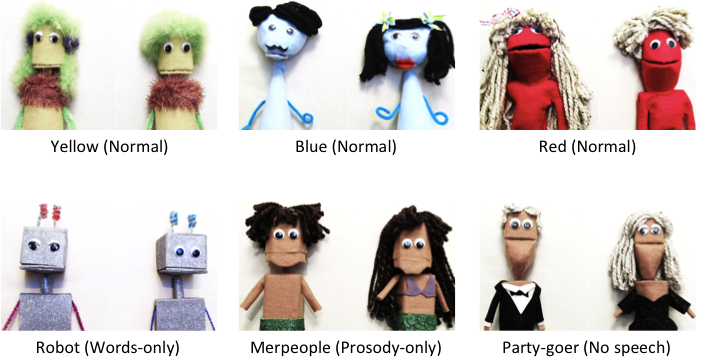
\includegraphics[width=0.9\textwidth]{figures/FIG-EN-stim.png}
\end{center}
\caption{The six puppet pairs (and associated audio conditions). Each pair was linked to three distinct conversations from the same condition across the three experiment versions.}
\label{fig:puppets}
\end{figure}

\subsubsection{Materials}
We created 18 short videos of improvised, child-friendly conversation (Figure \ref{fig:puppets}). To eliminate non-verbal cues to turn transition and to control the types of linguistic information available in the stimuli we first audio-recorded improvised conversations, then phonetically manipulated those recordings to limit the availability of prosodic and lexical information, and finally recorded video to accompany the manipulated audio, featuring puppets as talkers. 

\textit{Audio recordings}. The recording session was set up in the same way as the first experiment, but with a shorter warm up period (5--10 minutes) and a pre-determined topic for the child-friendly improvisation (`riding bikes', `pets', `breakfast', `birthday cake', `rainy days', or `the library'). All of the talkers were native English speakers, and were recorded in male-female pairs. As before, we asked talkers to speak ``as if they were on a children's television show'' and to ask at least a few questions during the improvisation. We cut each audio recording down to the 20-second interval with the most turn activity. The 20-second clips were then phonetically manipulated and used in the final video stimuli.

\textit{Audio Manipulation}. We created four versions of each audio clip: \textit{Normal}, \textit{words only}, \textit{prosody only}, and \textit{no speech}. That is, one version with a full linguistic signal (\textit{normal}), and three with incomplete linguistic information (hereafter ``limited cue'' conditions). The \textit{normal} clips were the unmanipulated, original audio clips. 

The \textit{words only} clips were manipulated to have robot-like speech: We flattened the intonation contours to each talker's average pitch (F0) and we reset the duration of every nucleus and coda to each talker's average nucleus and coda duration.\footnote{We excluded hyper-lengthened words like [w\textipa{aU:}] `woooow!'. These were rare in the clips.} We made duration and pitch manipulations using PSOLA resynthesis in Praat \citep{Praat}. Thus, the \textit{words only} versions of the audio clips had no pitch or durational cues to upcoming turn boundaries, but did have intact lexicosyntactic cues (and residual phonetic correlates of prosody, e.g., intensity). 

We created the \textit{prosody only} clips by low-pass filtering the original recording at 500 Hz with a 50 Hz Hanning window (following de Ruiter et al., 2006). This manipulation creates a ``muffled speech'' effect because low-pass filtering removes most of the phonetic information used to distinguish between phonemes. The \textit{prosody only} versions of the audio clips lacked lexical information, but retained their intonational and rhythmic cues to upcoming turn boundaries. 

The \textit{no speech} condition served as a non-linguistic baseline. For this condition, we replaced the original clip with multi-talker babble: We overlaid different child-oriented conversations (not including the original one), and then cropped the result to the duration of the original video. Thus, the \textit{no speech} audio clips lacked any linguistic information to upcoming turn boundaries---the only cue to turn taking was the opening and closing of the puppets' mouths. 

Finally, because low-pass filtering removes significant acoustic energy, the \textit{prosody only} clips were much quieter than the other three conditions. Our last step was to downscale the intensity of the audio tracks in the three other conditions to match the volume of the \textit{prosody only} clips. We referred to the conditions as ``normal'', ``robot'', ``mermaid'', and ``birthday party'' speech when interacting with participants.

\textit{Video recordings}. We created puppet video recordings to match the manipulated 20-second audio clips. The puppets were minimally expressive; the experimenter could only control the opening and closing of their mouths; their head, eyes, arms, and body stayed still. Puppets were positioned looking forward to eliminate shared gaze as a cue to turn structure \citep{thorgrimsson2015}. We took care to match the puppets' mouth movements to the syllable onsets as closely as possible, specifically avoiding any mouth movement before the onset of a turn. We then added the manipulated audio clips to the puppet video recordings by hand.

We used three pairs of puppets used for the \textit{normal} condition---`red', `blue' and `yellow'---and one pair of puppets for each limited cue condition: ``robots'', ``merpeople'', and ``party-goers'' (Figure 8). We randomly assigned half of the conversation topics (`birthday cake', `pets', and `breakfast') to the \textit{normal} condition, and half to the limited cue conditions (`riding bikes', `rainy days', and `the library'). We then created three versions of the experiment, so that each of the six puppet pairs was associated with three different conversation topics across the different versions of the experiment (18 videos in total). We ensured that the position of the talkers (left and right) was counterbalanced in each version by flipping the video and audio channels as needed.

% PART UNFINISHED: can add a link at the end of the prior paragraph to video examples

The duration of turn transitions and the number of speaker changes across videos was variable because the conversations were recorded semi-spontaneously. We measured turn transitions from the audio recording of the \textit{normal}, \textit{words only}, and \textit{prosody only} conditions. There was no audio from the original conversation in the \textit{no speech} condition videos, so we measured turn transitions from the video recording, using ELAN video editing software \citep{ELAN}. 

% PART UNFINISHED: update gap information
There were 85 turn transitions for analysis after excluding transitions longer than 550 msec and shorter than 90 msec. The remaining turn transitions had slightly more questions than non-question (N$=$50 and N$=$35, respectively), with transitions distributed somewhat evenly across conditions (keeping in mind that there were three \textit{normal} videos and only one limited cue video for each experiment version): \textit{Normal} (N$=$36), \textit{words only} (N$=$13), \textit{prosody only} (N$=$17), and {no speech} (N$=$19). Inter-turn gaps for questions (mean$=$365, median$=$427) were longer than those for non-questions (mean$=$302, median$=$323) on average, but gap duration was overall comparable across conditions: \textit{Normal} (mean$=$334, median$=$321), \textit{words only} (mean$=$347, median$=$369), \textit{prosody only} (mean$=$365, median$=$369), and \textit{no words} (mean$=$319, median$=$329). The longer gaps for question transitions could give them an advantage because our anticipatory measure includes shifts initiated during the gap between turns (Figure \ref{fig:criterion}).

\subsection{Procedure}
We used the same experimental apparatus and procedure as in the first experiment. Each participant watched six puppet videos in random order, with five 15--30 second filler videos placed in-between (e.g., running puppies, moving balls, flying bugs). Three of the puppet videos had \textit{normal} audio while the other three had \textit{words only}, \textit{prosody only}, and \textit{no speech} audio. This experiment required no special instructions so the experimenter immediately began each session with calibration (same as before) and then stimulus presentation. The entire experiment took less than five minutes.

\subsubsection{Data preparation and coding}
We coded each turn transition for its linguistic condition (\textit{normal}, \textit{words only}, \textit{prosody only}, and \textit{no speech}) and transition type (question/non-question)\footnote{We coded \textit{wh-}questions as ``non-questions'' for the \textit{prosody only} videos. Polar questions had a final rising prosodic contour, but \textit{wh-}questions did not  \citep{hedberg2010}.} and identified anticipatory gaze switches to the upcoming speaker using the methods from Experiment 1.

\subsection{Results}
\label{sec:results2}

Participants' pattern of gaze indicated that they performed basic turn tracking across all ages and in all conditions. Participants looked at the screen most of the time during video playback (82\% and 86\% average for children and adults, respectively). Children and adults primarily kept their eyes on the person who was currently speaking: They gazed at the current speaker between 44\% and 69\% of the time, looking back at the addressee between 11\% and 14\% of the time (Table 2). They tracked the current speaker in every condition---even one-year-olds looked more at the current speaker than at anything else in the three limited cue conditions (40\% for \textit{words only}, 43\% for \textit{prosody only}, and 39\% for \textit{no speech}). There was a steady overall increase in looks to the current speaker with age and added linguistic information (Tables \ref{tab:look_e2} and \ref{tab:look_e2b}). Looks to the addressee also decreased with age, but the change was minimal. 

\begin{table}[h]
\begin{center}
  \begin{tabular}{llcccc}
    \hline
    Age group & Speaker & Addressee & Other onscreen & Offscreen\\ 
    \hline
    1 & 0.44 & 0.14 & 0.23 & 0.19 \\ 
    2 & 0.50 & 0.13 & 0.24 & 0.14 \\ 
    3 & 0.47 & 0.12 & 0.25 & 0.16 \\ 
    4 & 0.48 & 0.11 & 0.29 & 0.12 \\ 
    5 & 0.54 & 0.11 & 0.20 & 0.14 \\ 
    6 & 0.60 & 0.12 & 0.18 & 0.10 \\
    Adult & 0.69 & 0.12 & 0.09 & 0.10 \\
%   Overall & 0.53 & 0.12 & 0.21 & 0.13 \\
    \hline
  \end{tabular}
\end{center}
  \caption{Average proportion of gaze to the current speaker and addressee during periods of talk across ages.}
\label{tab:look_e2}
\end{table}

\begin{table}[h]
\begin{center}
  \begin{tabular}{llcccc}
    \hline
    Condition & Speaker & Addressee & Other onscreen & Offscreen\\ 
    \hline
    Normal & 0.58 & 0.12 & 0.17 & 0.13 \\ 
    Words only & 0.54 & 0.11 & 0.24 & 0.10 \\ 
    Prosody only & 0.48 & 0.12 & 0.26 & 0.15 \\ 
    No speech & 0.44 & 0.13 & 0.26 & 0.18 \\
    \hline
  \end{tabular}
\end{center}
  \caption{Average proportion of gaze to the current speaker and addressee during periods of talk across conditions.}
\label{tab:look_e2b}
\end{table}

% Average prop gaze to the current speaker across conditions for one-year-olds
%                           speaker addressee other-screen offscreen
%Normal   		  0.4737582 0.1366432    0.2003952 0.1892035
%Words only    0.3977261 0.1283417    0.3112005 0.1627317
%Prosody only 0.4290202 0.1611453    0.2558657 0.1539688
%No speech    0.3786925 0.1228615    0.2356423 0.2628037

\begin{table}[h!]
\begin{center}
  \begin{tabular}{lcccl}
  \textbf{\textit{Children}} &&&& \\
    \hline
                       & Estimate & Std. Error & z value & Pr($>$$|$z$|$)    \\
    \hline
    (Intercept)                & -3.57414  &   0.48576 &  -7.358 & 1.87e-13 ***    \\
    Age                         & 0.02543 &    0.10260  &  0.248   & 0.8042        \\
    Condition$=$\textit{muffled}         &   -1.63429  &   0.86390 &  -1.892   & 0.0585 .      \\
    Condition$=$\textit{normal}            &  0.36710 &    0.43296 &   0.848  &  0.3965        \\
    Condition$=$\textit{robot}            &  -0.26741 &    0.59071 &  -0.453  &  0.6508        \\
    Type$=$\textit{non-Question}                      & -0.81873  &   0.59985 &  -1.365  &  0.1723        \\
    Duration                   &  4.17672  &   0.62446  &  6.689 & 2.25e-11 ***    \\
    Age*Condition$=$\textit{muffled}       &   0.39317 &     0.18907 &   2.080  &  0.0376 *      \\
    Age*Condition$=$\textit{normal}       &   0.12919 &    0.10227  &  1.263  &  0.2065        \\
    Age*Condition$=$\textit{robot}           &   0.13740  &   0.13568   & 1.013  &  0.3112        \\
    Age*Type$=$\textit{non-Question}                &    0.15116   &  0.13643  &  1.108  &  0.2679        \\
    Condition$=$\textit{muffled}*     &  1.77190  &   1.24864  &  1.419 &   0.1559        \\
    Type$=$\textit{non-Question} &&&& \\
    Condition$=$\textit{normal}*     &   0.91059  &   0.72095  &  1.263 &   0.2066        \\
    Type$=$\textit{non-Question} &&&& \\
    Condition$=$\textit{robot}*     &   -1.02193  &   1.01227  & -1.010  &  0.3127        \\
    Type$=$\textit{non-Question} &&&& \\
    Age*Condition$=$\textit{muffled}* &  -0.47057 &    0.28703 &  -1.639 &   0.1011        \\
    Type$=$\textit{non-Question} &&&& \\
    Age*Condition$=$\textit{normal}* &   -0.37542  &   0.16963  & -2.213 &   0.0269 *      \\
    Type$=$\textit{non-Question} &&&& \\
    Age*Condition$=$\textit{robot}*  &   0.08946  &   0.22349   & 0.400 &   0.6890        \\
    Type$=$\textit{non-Question} &&&& \\
    \hline
  &&&& \\
  \textbf{\textit{Adults}} &&&& \\
    \hline
                       &  Estimate & Std. Error & z value & Pr($>$$|$z$|$) \\    
    \hline
    (Intercept)           &  -3.4557   &   0.7199 &  -4.800 & 1.58e-06 *** \\ 
    Condition$=$\textit{muffled}     &     0.3349  &    0.8965  &  0.374 & 0.708692     \\ 
    Condition$=$\textit{normal}    &      1.2556   &   0.5633  &  2.229 & 0.025805 *   \\ 
    Condition$=$\textit{robot}       &     1.5938  &    0.7208 &   2.211 & 0.027023 *   \\ 
    Type$=$\textit{non-Question}                  &   0.4292  &    0.6089  &  0.705 & 0.480916     \\ 
    Duration             &     4.7500   &   1.2480  &  3.806 & 0.000141 *** \\ 
    Condition$=$\textit{muffled}*  &  0.6627  &    1.2138 &   0.546 & 0.585108     \\ 
    Type$=$\textit{non-Question} &&&& \\
    Condition$=$\textit{normal}* &   -0.9452  &    0.7631 &  -1.239 & 0.215475     \\ 
    Type$=$\textit{non-Question} &&&& \\
    Condition$=$\textit{robot}*   &  -1.1265  &    0.9109  & -1.237 & 0.216201     \\ 
    Type$=$\textit{non-Question} &&&& \\
    \hline
  \end{tabular}
\end{center}
  \caption{Model output for children and adults' anticipatory gaze switches.}
\label{tab:E2-models}
\end{table}

\subsubsection{Statistical models}
\label{sec:models2}

We identified anticipatory gaze switches for all 85 usable turn transitions, and analyzed them for effects of language condition, transition type, and age with two mixed-effects logistic regressions \citep{lme4, R}. We again built separate models for children and adults because effects of age were only pertinent to the children's data. The child model included condition (normal/prosody only/words only/no speech; with no speech as the reference level), transition type (question vs. non-question), age (1, 2, 3, 4, 5, 6), and duration of the inter-turn gap (in seconds) as predictors, with full interactions between language condition, transition type, and age.  We again included the duration of the inter-turn gap as a control predictor and added random effects of item (turn transition) and participant, with random slopes of transition type for participants \citep{barr2013}. The adult model included condition, transition type, their interactions, and duration as a control predictor, with participant and item included as random effects and random slopes of condition and transition type.

Children's anticipatory gaze switches showed an effect of gap duration (\textit{$\beta$}=4.18, \textit{SE}=0.624, \textit{t}=6.689, \textit{p}$<$.001), a two-way interaction of age and language condition (for prosody only speech compared to the no speech reference level; \textit{$\beta$}=0.393, \textit{SE}=0.189, \textit{t}=2.08, \textit{p}$<$.05), and a three-way interaction of age, transition type, and language condition (for normal speech compared to the no speech reference level; \textit{$\beta$}=-0.375, \textit{SE}=0.17, \textit{t}=-2.213, \textit{p}$<$.05). There were no significant effects of age or transition type alone (Table \ref{sec:models2}), with only a marginal effect of language condition (for prosody only compared to the no speech reference level; \textit{$\beta$}=-1.634, \textit{SE}=0.864, \textit{t}=-1.89, \textit{p}$=$.06)

Adults' anticipatory gaze switches showed effects of gap duration (\textit{$\beta$}=4.75, \textit{SE}=1.248, \textit{t}=3.806, \textit{p}$<$.001) and language condition (for normal speech \textit{$\beta$}=1.256, \textit{SE}=0.563, \textit{t}=2.229, \textit{p}$<$05. and words only speech \textit{$\beta$}=1.594, \textit{SE}=0.721, \textit{t}=2.211, \textit{p}$<$.05  compared to the no speech reference level). There were no effects of transition type (\textit{$\beta$}=0.429, \textit{SE}=0.609, \textit{t}=0.705, \textit{p}$=$.48).

\begin{figure}[h!]
  \centering
  \subfloat[Children]{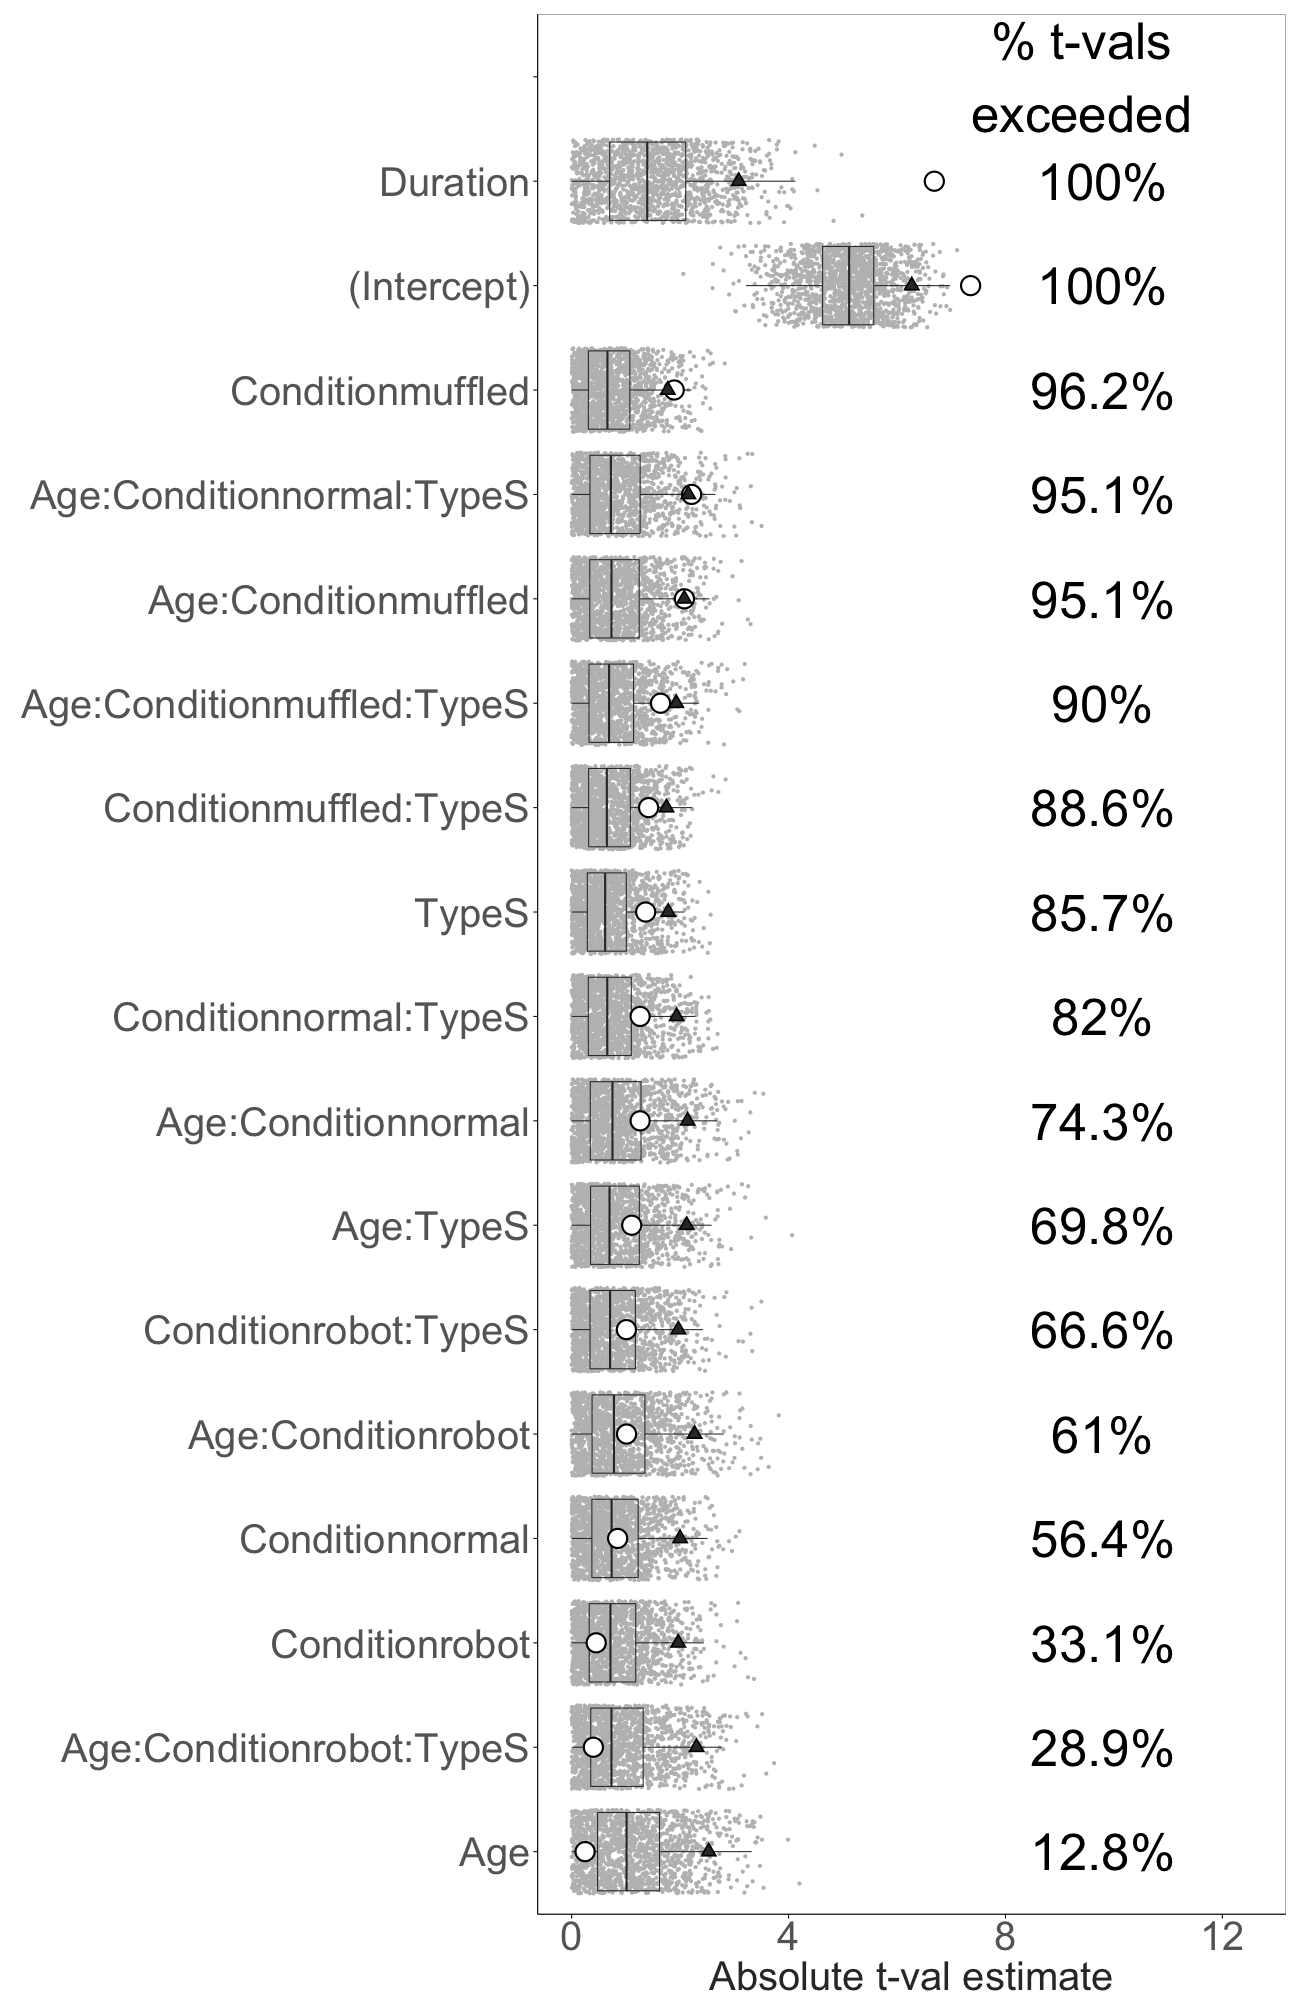
\includegraphics[width=0.49\textwidth]{figures/E2-chi-randrun-t-vals-absolute.png}\label{fig:E2-ChiTs}}
  \hfill
  \subfloat[Adults]{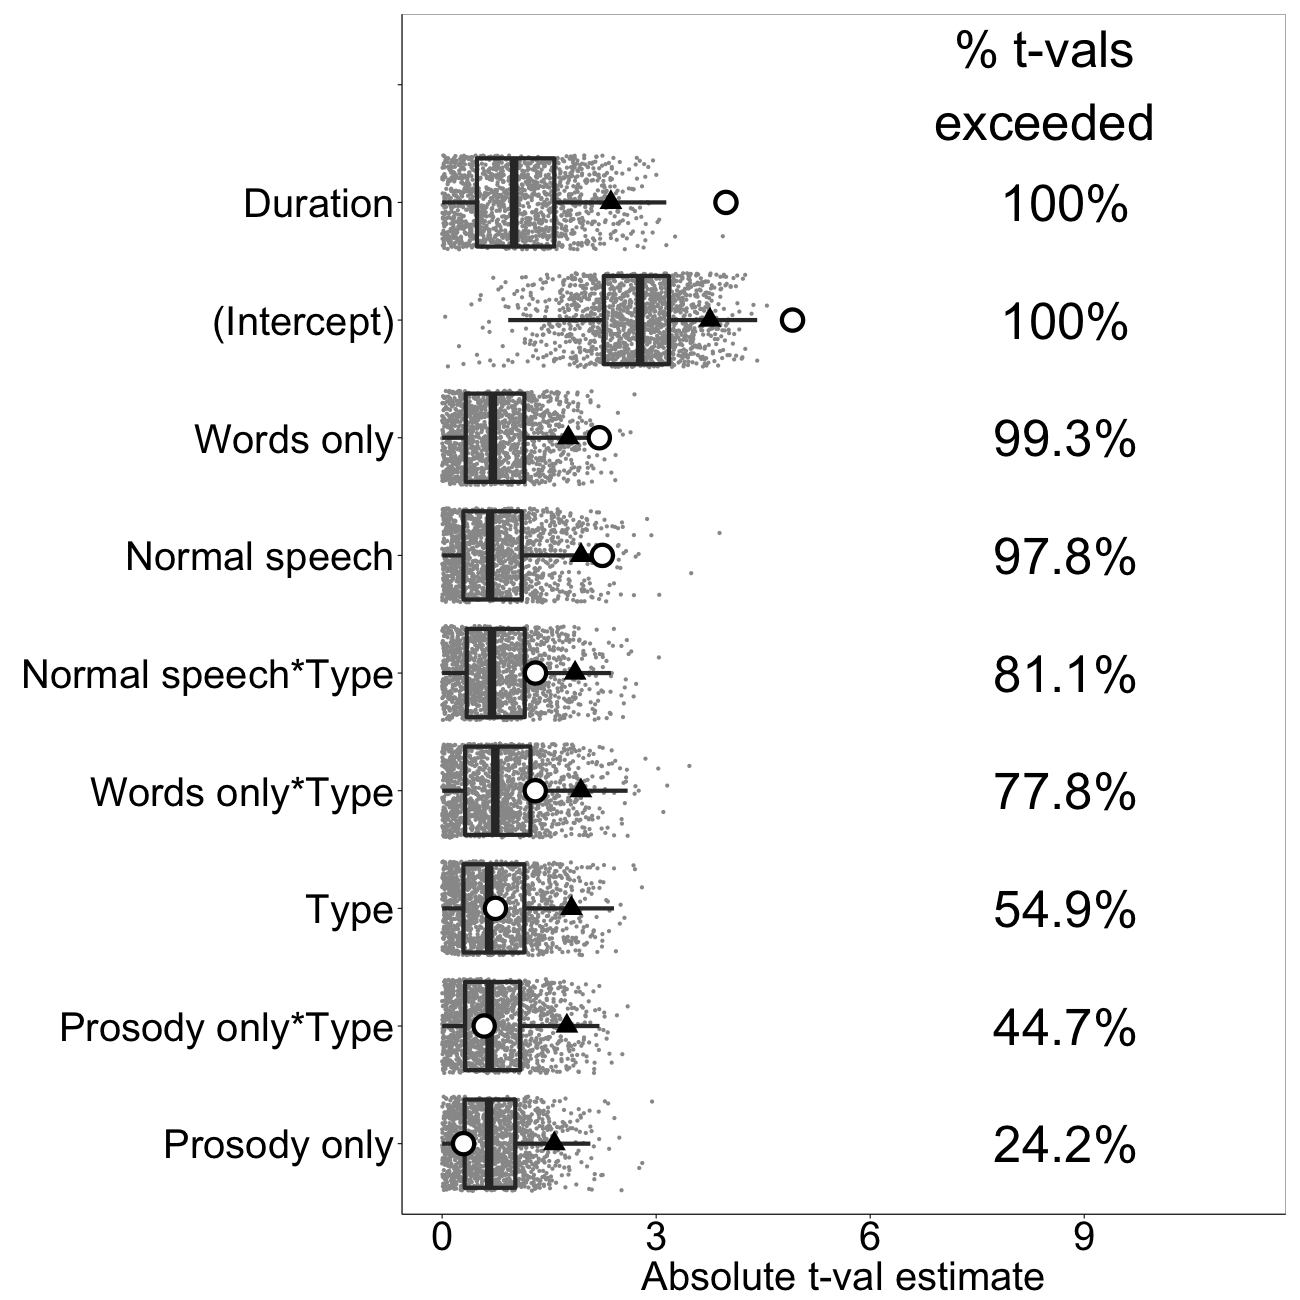
\includegraphics[width=0.49\textwidth]{figures/E2-adu-randrun-t-vals-absolute.png}\label{fig:E2-AduTs}}
  \caption{Random-permutation and original $|$\textit{t}-values$|$ for predictors of children and adults' anticipatory gaze rates. Gray dots $=$ random model estimates, White dots $=$ original model estimates, Triangles $=$ 95th percentile for each \textit{t}-value distribution.}
\end{figure}

\subsubsection{Random baseline comparison}
\label{sec:randbaseline2}

Using the same technique described in experiment 1 (Section \ref{sec:randbaseline1}), we created and modeled 5,000 random permutations of participants' anticipatory gaze. Our baseline analyses revealed that none of the significant predictors from models of the original, turn-related data (Table \ref{tab:E2-models}: Children) can be explained by random looking. In the children's data, the original model's \textit{t}-values for language condition (prosody only), gap duration, the two-way interaction of age and language condition (prosody only) and the three-way interaction of age, transition type, and language condition (normal speech) were all greater than 95\% of the randomly permuted \textit{t}-values (96.2\%, 100\%, 95.1\%, and 95.1\%, respectively; Figure \ref{fig:E2-ChiTs}). Similarly, the adults' data showed significant differentiation from the randomly permuted data for all originally significant predictors: gap duration and language condition for normal speech and words-only speech (greater than 100\%, 96.8\%, and 98.7\% of random \textit{t}-values, respectively; Figure \ref{fig:E2-AduTs}). The effects of language condition and transition type for the real and randomly permuted data can also be observed in Figure \ref{fig:E1-randvsreal}.

% PART UNFINISHED (potentially)
% We excluded the output of random-permutation models that did not converge to remove unreliable model results from our percentile calculations below (XX\% and XX\% of models for children and adults, respectively). 

\begin{figure}[h]
\begin{center}
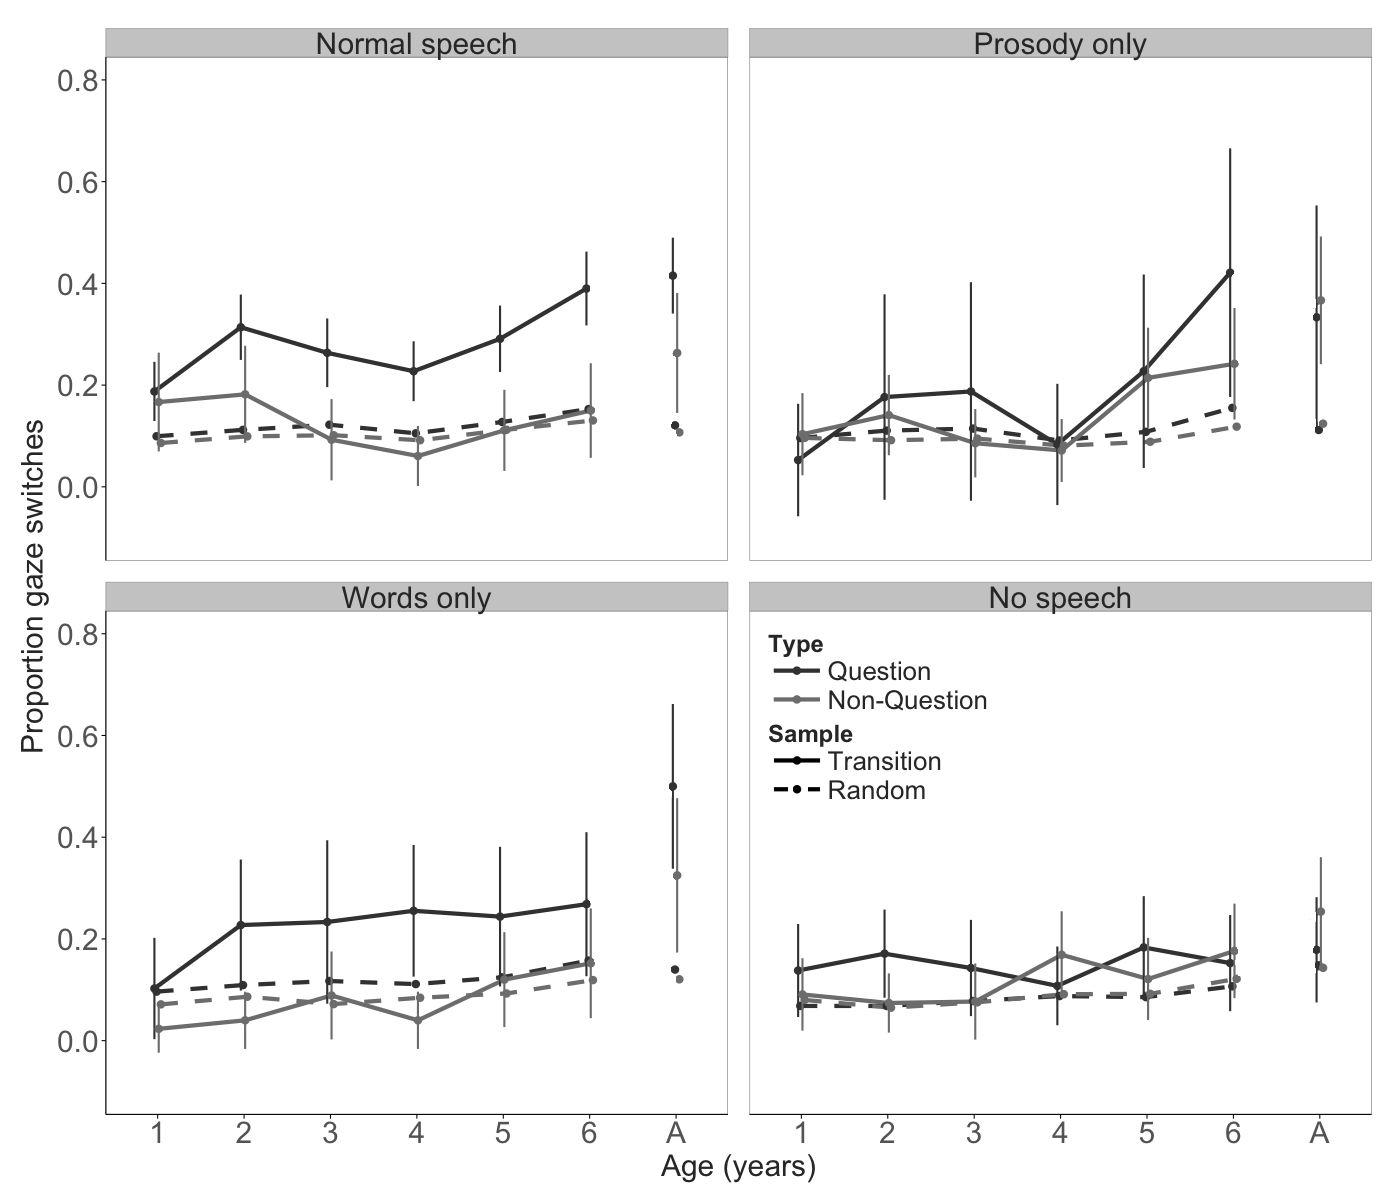
\includegraphics[width=0.9\textwidth]{figures/E2-samples-by-lang-groups-trans-types.png}
\end{center}
\caption{Anticipatory gaze rates across language condition and transition type for the real (blue, dark green, light green, and red) and randomly permuted (gray) data. Vertical bars represent the standard error.} 
\label{fig:E2-randvsreal}
\end{figure}

\begin{figure}[h!]
\begin{center}
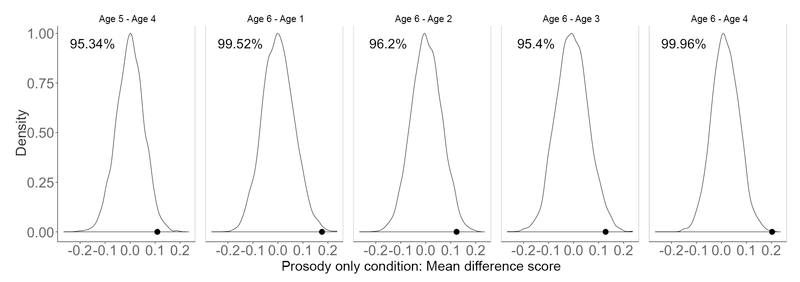
\includegraphics[width=0.9\textwidth]{figures/E2-child-randvsreal-ttest-muffledages.png}
\end{center}
\caption{Significant pairwise comparisons of the prosody only-no speech linguisitic condition effect, across ages, for the original data (black dots) and the 5,000 randomly permuted datasets (distribution).} 
\label{fig:E2-lgageinteraction}
\end{figure}

\begin{figure}[h!]
\begin{center}
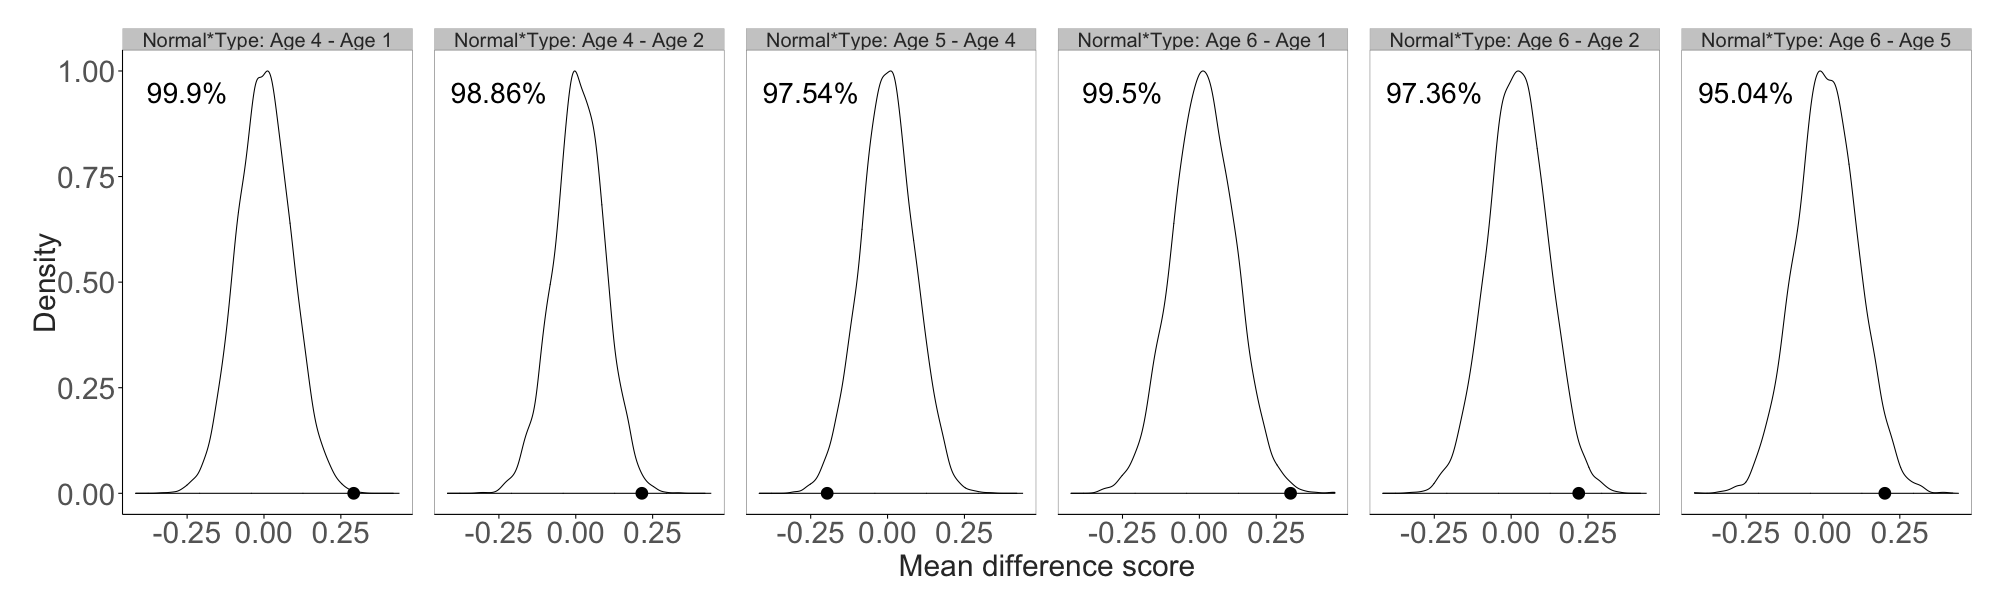
\includegraphics[width=0.9\textwidth]{figures/E2-child-randvsreal-ttest-normaltypesages.png}
\end{center}
\caption{Significant pairwise comparisons of the normal speech-no speech language condition effect for questions status, across ages, for the original data (black dots) and the 5,000 randomly permuted datasets (distribution).} 
\label{fig:E2-lgagetypeinteraction}
\end{figure}

\paragraph{Developmental effects}
The model of the children's data revealed two significant interactions with age, neither of which derived from random looking (Table \ref{tab:E2-models}; Figure \ref{fig:E2-randvsreal}). The first was a significant interaction of age and language condition (for prosody only compared to the no speech reference level), suggesting a different age effect between the two linguistic conditions. As in Experiment 1, we further explored the age effect by extracting the average difference score over subjects for this age-language condition interaction in each random permutation of the data, making pairwise comparisons between the six age groups. Figure \ref{fig:E2-lgageinteraction} shows the comparisons that demonstrate a significant difference in age for the no speech baseline vs. the prosody only condition, revealing that anticipatory gaze in the prosody only condition significantly improves with age, especially at ages 5 and 6 (all with difference scores greater than 95\% of the random data scores; \textit{p} $<$ .05).

The second interaction with age was a three-way interaction of age, transition type, and language condition (for normal speech compared to the no speech baseline). We again created pairwise comparisons of the average difference scores for this age-transition type-language condition interaction in each random permutation of the data, with significant differences shown in Figure \ref{fig:E2-lgagetypeinteraction}. These pairwise comparisons showed that the effect of transition type in the normal speech condition became larger with age, with significant improvements by age 4 over ages 1 and 2 (99.9\% and 98.86\%, respectively), by age 5 over age 4 (97.54\%), and by age 6 over ages 1, 2, and 5 (99.5\%, 97.36\%, and 95.04\%), all significantly different from chance (\textit{p} $<$ .05).

\subsection{Discussion}
\label{sec:discussion2}
As in Experiment 1, children and adults spontaneously tracked the turn structure of the conversations, making anticipatory gaze switches at an above-chance rate across all ages but not in all conditions (Table \ref{tab:e2_look}; Figure \ref{fig:E2-randvsreal}). In the normal speech condition, however, when children had access to full linguistic information, they made more anticipatory gaze switches than expected by chance even at age one. Children's anticipatory gaze rates were affected by gap duration, plus interactions of language condition, transition type and age (Table \ref{tab:E2-models}), none of which could be explained by a baseline of random gaze switching (Figure \ref{fig:E2-ChiTs}).

Two of the three linguistic conditions affected children's anticipatory gaze switches, compared to the no-speech reference level: prosody-only speech and normal speech. Prosody only speech resulted in fewer anticipatory gazes overall, compared to the no-speech baseline, though the effect was only marginal (\textit{p}$=$.06). However, prosody-only speech \textit{did} significantly differ from the no speech condition in its interaction with age: whereas age gains were negligible in the no speech condition, 5- and 6-year-olds in the prosody-only condition showed significantly more anticipatory gaze switches than younger children (Figure \ref{fig:E2-lgageinteraction}), going from below- and at-chance anticipatory gaze rates to being well above chance (Figure \ref{fig:E2-randvsreal}).

The normal speech condition showed a significantly more gains in anticipatory gaze for questions with age compared to the no-speech condition. As in Experiment 1, children consistently made more anticipatory gazes after hearing questions when they had access to lexical material. But now, with a larger age span in Experiment 2, we can begin to see a developmental path for the question effect. At least for normal speech, greater anticipatory looking for questions is not present from the start: 4-year-olds are the first to make significant gains on 1- and 2-year-olds, but then there are further significant gains at age 5, and again age 6 (Figure \ref{fig:E2-lgagetypeinteraction}). While children at ages five and six showed adult-like differentiation of questions and non-questions in the normal speech condition, 1-year-olds had nearly identical switch rates for the two transition types. This suggests that the participants' tendency to make more anticipatory switches for questions emerges after age one and continues developing, with rapid gains in ages three through age six. Finally, children showed a straightforward effect of gap duration (Table \ref{tab:E2-models}), as in Experiment 1.

Adults' anticipatory gaze rates were affected by gap duration and two of the language conditions (Table \ref{tab:E2-models}), none of which could be explained by a baseline of random gaze switching (Figure \ref{fig:E2-AduTs}). Adults made more anticipatory switches overall for the normal speech and words-only conditions compared to the no-speech condition, falling in-line with past work showing that adults primarily use lexical information in making predictions about upcoming turn structure \citep{de-ruiter2006}. Though adults did make more anticipatory switches for questions than non-questions on average in the two lexical conditions (Figure \ref{fig:E2-randvsreal}), the effect of transition type was not significant in either (Table \ref{tab:E2-models}), unlike Experiment 1. Like children, adults also showed a straightforward effect of gap duration.

\subsubsection{Summary}
\label{sec:summary2}

%We identified anticipatory gaze switches for all 79 usable turn transitions using the same criteria as in Experiment 1. We expected to see the most anticipatory switches in the \textit{normal} condition and the least anticipatory switches in the \textit{no speech} condition because they contained the most and least linguistic information, respectively. We expected to replicate our finding that questions result in more anticipatory switches than non-questions, with the added hypothesis that the question effect is driven by lexicosyntactic cues. We also anticipated an overall increase in anticipatory switches with age. Finally, since the development of prosodic skills partially precedes the development of lexicosyntax, we expected to see more switches in the \textit{prosody only} condition compared to the \textit{words only} condition in the youngest age groups.
%
%We found that participants at all ages made anticipatory gaze switches more often than would be expected by chance in almost all conditions, but sometimes by a small margin (Figure \ref{fig:randvsrealEN}). For example, anticipatory switches in the \textit{no speech} videos were often modestly above chance (with the exception of 5- and 6-year-olds). One interpretation of this finding is that children do not use linguistic information to predict upcoming turns---the only cue to turn taking in the \textit{no speech} condition was the alternating mouth movements of the conversing puppets. With sufficiently long inter-turn gaps, participants could simply switch their gaze to the responder when the prior talker finishes talking---a strategy that doesn't rely on linguistic information. But this interpretation is not compatible with our the effects of linguistic information that do emerge in the data: An early advantage for prosody and a later advantage for lexical question cues.
%
%We saw a generalize early advantage for prosody over lexicosyntax in children's spontaneous turn predictions. Notably, while children performed well with \textit{prosody only} speech from the start, they seemed to only reliably exceed chance in the \textit{words only} condition at ages three and older. By age three, the general advantage for prosody over lexicosyntax seems to disappear with more equal rates of switching overall for the two partial linguistic conditions.
%
%\begin{figure}[t]
%\begin{center}
%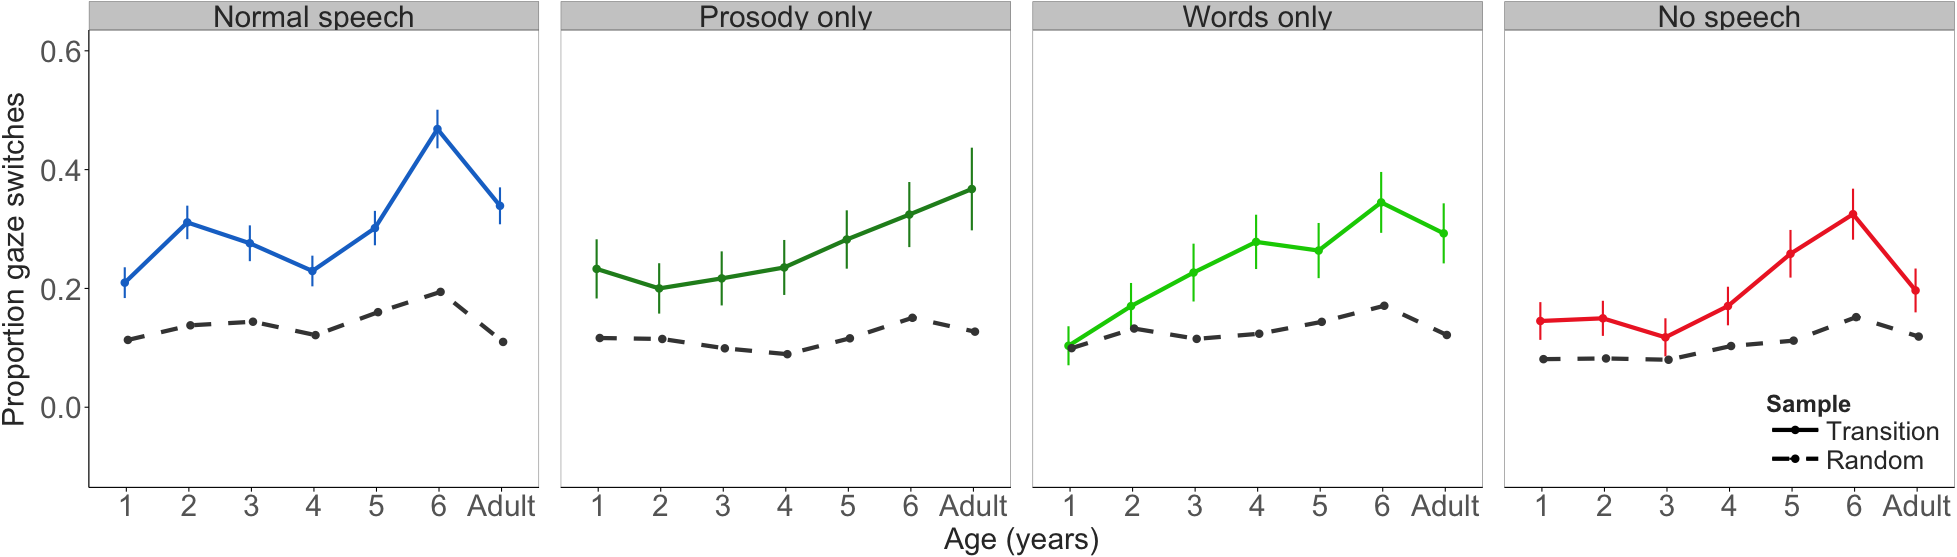
\includegraphics[width=0.99\textwidth]{figures/FIG-randvsreal-EN.png}
%\end{center}
%\caption{Baseline-corrected proportion of anticipatory gaze switches made for actual (solid) and randomly-shuffled (dashed) turn transitions in each condition, and across ages. Error bars represent the standard error of the mean.} 
%\label{fig:randvsrealEN}
%\end{figure}
%
%We observed that, overall, children and adults made the fewest anticipatory switches in the \textit{no speech} videos (9\%) and the most in the \textit{normal} videos (16\%), with the \textit{prosody only} and \textit{words only} videos falling in-between (14\% and 11\%, respectively; Figure \ref{fig:conditionsEN}). However, these condition-based differences were primarily driven by transition type effects (question vs. non-question).
%
%\begin{figure}[t]
%\begin{center}
%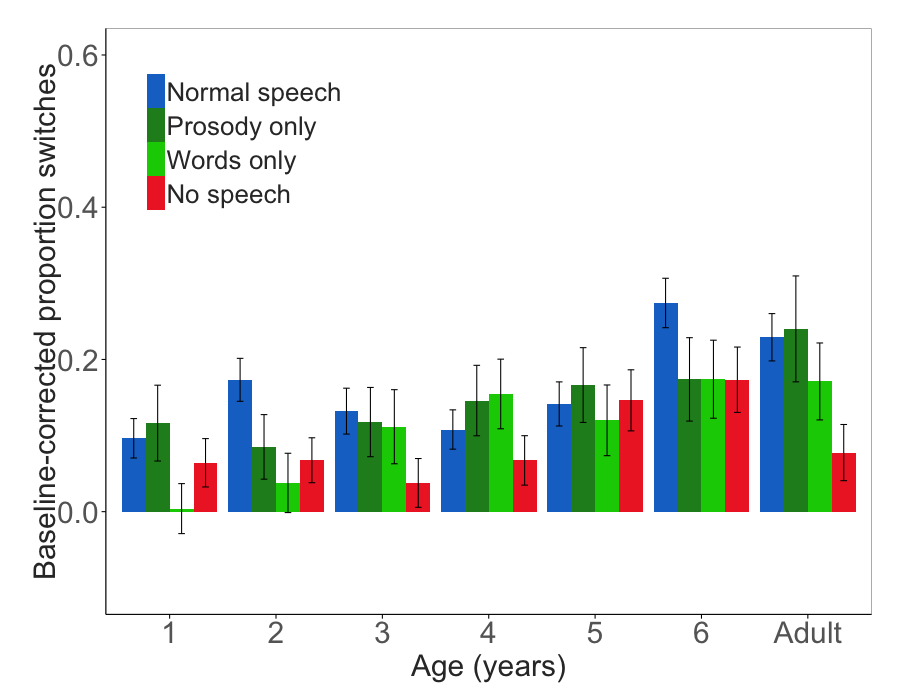
\includegraphics[width=0.65\textwidth]{figures/FIG-conditions-EN.png}
%\end{center}
%\caption{Baseline-corrected proportion of anticipatory gaze switches made for turn transitions in each speech condition, and across ages. Error bars represent the standard error of the mean.} 
%\label{fig:conditionsEN}
%\end{figure}
%
%As in Experiment 1, we made condition, age and transition type comparisons based on baselin-corrected switching values; we corrected each participant's gaze data by subtracting their random baseline from their actual switching for each turn transition.
%
%We found that participants made more anticipatory gaze switches following questions than non-questions, but only in the two lexical conditions (\textit{normal} and \textit{words only} speech). The advantage for questions was strongest in the \textit{normal} speech condition, where it emerged early in development. The question effect became larger with age in both lexical conditions. While children made small, sometimes non-linear, gains in their anticipatory switches for non-questions as they grew older, they made large gains in their anticipatory switches with age (especially between ages one and two; Figure \ref{fig:questionsEN}). The increased switching for questions between ages one to two indicates that, around this age, children begin to leverage lexicosyntactic cues in the speech signal to identify questions in ongoing conversation. In the lexical conditions, children had access to early cues to questionhood, such as \textit{wh}-words and subject-auxiliary inversion, to predict an upcoming speaker change. In the \textit{normal} condition, where the question effect was strongest, lexical and syntactic cues were reinforced by question prosody for polar questions.
%
%\begin{figure}[t]
%\begin{center}
%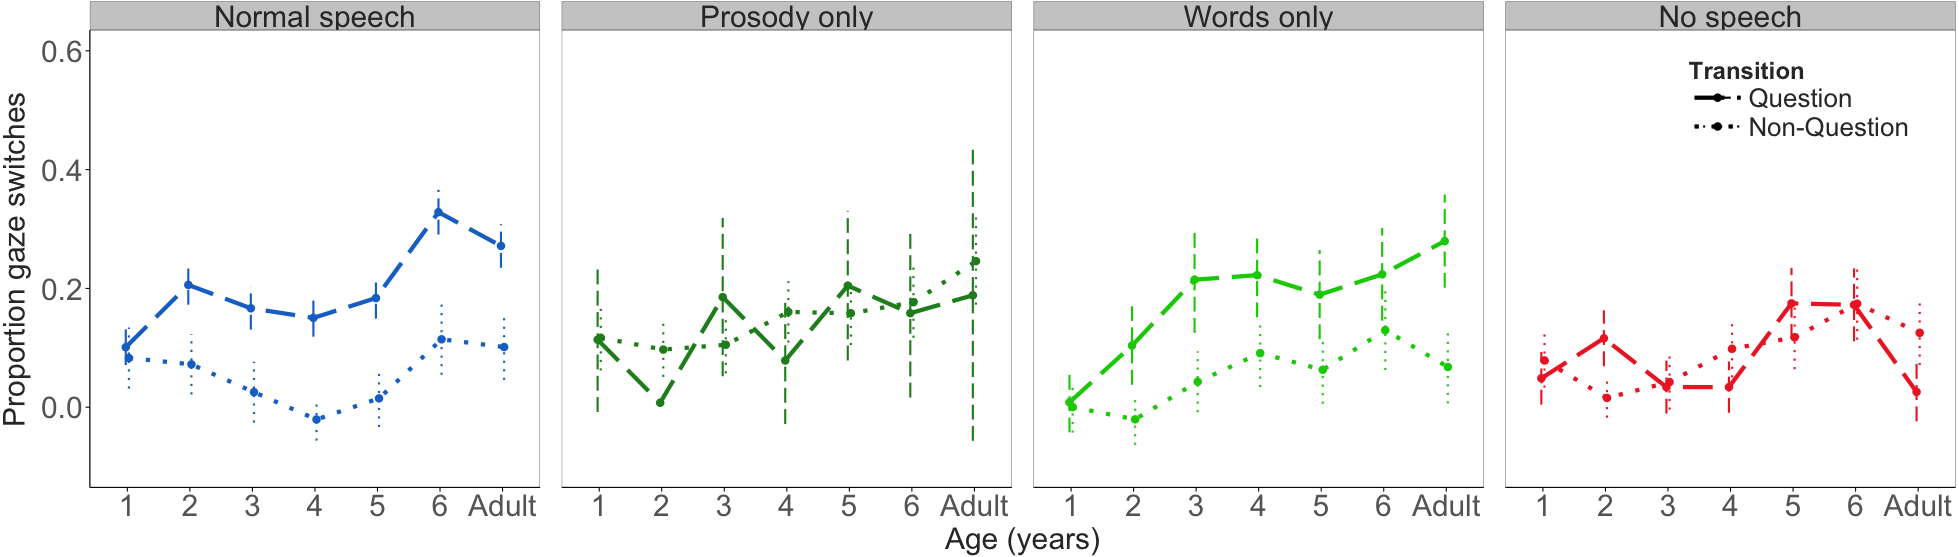
\includegraphics[width=0.99\textwidth]{figures/FIG-QvsNQ-EN.png}
%\end{center}
%\caption{Baseline-corrected proportion of anticipatory gaze switches made for question- (dashed) and non-question- (dotted) turn transitions in each condition, and across ages. Error bars represent the standard error of the mean.} 
%\label{fig:questionsEN}
%\end{figure}
%
%Children showed increased anticipatory switching with age across all conditions, making almost as many transitions as adults by ages five and six. Adults reacted to the \textit{no speech} condition differently than the children did, tracking the interaction less closely than in the three linguistic conditions. They may have minimized switching in the \textit{no speech} condition because they realized that there was no conversation to follow.
%
%\subsubsection{Statistical analysis}
%
%We tested these findings in two linear mixed-effects models of participants' baseline-corrected anticipatory switches---one model each for children and adults. The child model included condition (\textit{normal}, \textit{words only}, \textit{prosody only}, and \textit{no speech}; \textit{normal} in the intercept), transition type (question vs. non-question), age, and gap duration as fixed effects, with full interactions between condition, transition type, and age. The model also included random effects of item (turn transition) and participant, with random slopes of condition and transition type for participants. The adult model matched the child model, excluding age-related effects.
%
%There was a significant effect of gap duration. Children had time to make more anticipatory switches in analysis windows with longer gaps (\textit{$\beta$}=0.294, \textit{SE}=0.091, \textit{t}=3.231, \textit{p}$<$.01). An effect of gap duration is expected since prior work using spontaneous anticipatory switching has found that most switches occur in the inter-turn gap (Keitel et al., 2013; Hirvenkari, 2013; Tice and Henetz, 2011).
%
%The only effects of linguistic condition derived from interactions with age and transition type, despite large differences in the linguistic information available across conditions. (Figure \ref{fig:questionsEN}). The model of children's data confirmed two three-way effects of age, condition, and transition type. Children made significantly more anticipatory switches for questions with age in the \textit{normal} (\textit{$\beta$}=0.04, \textit{SE}=0.008, \textit{t}=5.168, \textit{p}$<$.001) and \textit{words only} conditions (\textit{$\beta$}=0.031, \textit{SE}=0.01, \textit{t}=3.170, \textit{p}$<$.01). Overall, they made a switch twice as often after hearing a question (16\%) than a non-question (8\%) in the \textit{words only} condition, and nearly four times as often in the \textit{normal} condition (19\% vs. 5\%). Since the question effect was limited to the lexical conditions, there was no effect of transition type. There were also no further interactions of age and condition, or of transition type and condition. There was, however, a significant two-way interaction of transition type and age (\textit{$\beta$}=-0.031, \textit{SE}=0.01, \textit{t}=-3.18, \textit{p}$<$.01) in addition to the three-way interactions for the \textit{normal} and \textit{words only} conditions already mentioned.
%
%Last but not least, we confirmed that children generally made more anticipatory switches as they got older: The model showed a significant effect of age (\textit{$\beta$}=0.028, \textit{SE}=0.009, \textit{t}=3.018, \textit{p}$<$.01). Though the increase in anticipatory looks with age came, in large part, from questions effects in the lexical conditions, children also showed increased switches for non-questions and non-lexical conditions. The increases related to non-questions and non-lexical conditions were overall smaller and sometimes followed a non-linear trajectory (Figure \ref{fig:questionsEN}). As in Experiment 1, early switches (planned before the end of the prior turn) did not show large increases with age, with adults making the fewest early switches in the three linguistic conditions (Figure \ref{fig:cumulativeEN}).
%
%\begin{figure}[ht]
%\begin{center}
%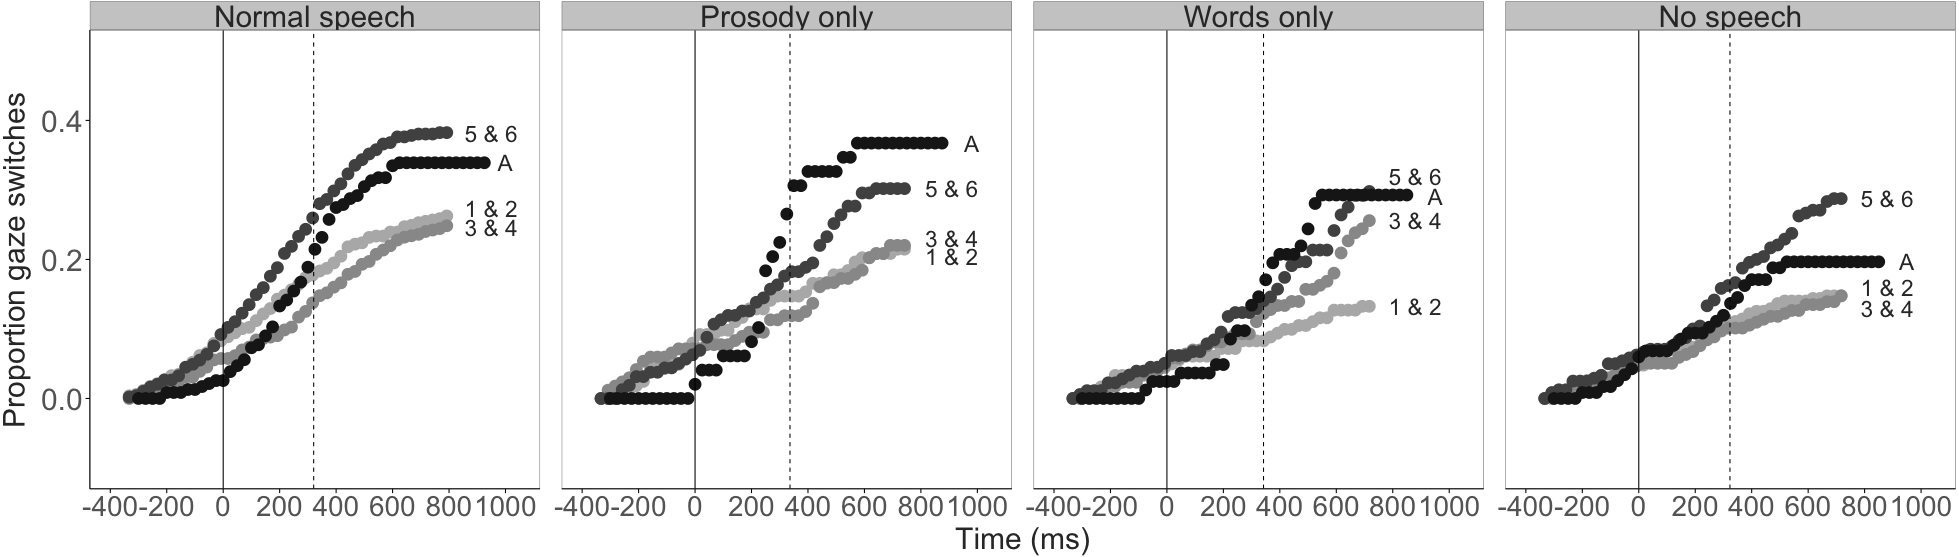
\includegraphics[width=0.99\textwidth]{figures/FIG-cumulative-EN.png}
%\end{center}
%\caption{Cumulative proportion of anticipatory gaze switches planned during the transition window, across conditions and ages. Age is indicated by hue (darker = older). The solid line is the offset of the pre-gap turn, and the dashed line is the median onset of the post-gap turn in each condition. ``Early switches'' occur before 0.} 
%\label{fig:cumulativeEN}
%\end{figure}
%
%The advantage for questions over non-questions in these results reinforces our findings from Experiment 1. They suggest that even two-year-olds can reliably distinguish questions from other transition types in third-party conversation, especially when full linguistic information is available. Inspecting the data more closely, we found that 43\% of one-year-olds made more anticipatory switches after questions than non-questions in the \textit{normal} condition, and 24\% of them did so in the \textit{words only} condition. Meanwhile, 61\% of two-year-olds show the effect in the \textit{normal} condition, and 52\% of them do in the \textit{words only} condition, which is already close to the average for older children and adults (Table \ref{tab:questioneffectexp2}).
%
%Our results suggest that the question effect emerges between ages one and two, but further testing is needed to establish whether this is the case. For example, the size and emergence of the question effect for various question types and question cues could differ (\textit{wh-} vs. \textit{yes-no}; early vs. late in the utterance), but we do not have enough data to make those distinctions in the current analysis. Also, 43\% of one-year-olds already showed more switching for questions than non-questions in the \textit{normal} speech condition---the only condition with the full range of linguistic cues children hear in everyday life. Future work with more fine-grained age samples and better controlled \textit{normal} speech might then find that children can identify questions in conversation even earlier.
%
%\begin{table}[t]
%\begin{center}
%  \begin{tabular}{ccc}
%    \hline
%    Age group & Normal speech & No speech \\ 
%    \hline
%    1 & 0.43 & 0.24 \\
%    2 & 0.61 & 0.52 \\
%    3 & 0.63 & 0.42 \\
%    4 & 0.78 & 0.52 \\
%    5 & 0.91 & 0.52 \\
%    6 & 0.75 & 0.50 \\
%    Adult & 0.67 & 0.57 \\
%    \hline
%  \end{tabular}
%\end{center}
%  \caption{Proportion of participants showing numerically more anticipatory switches for questions than non-questions in the \textit{normal} and \textit{words only} conditions.}
%\label{tab:questioneffectexp2}
%\end{table}
%
%Finally, we confirmed that young children showed a benefit for prosody over lexicosyntax. We conducted two \textit{post-hoc} \textit{t}-tests for children under three, comparing their anticipatory switching rate against their estimated random switching rate in the \textit{prosody only} and \textit{words only} conditions. We found that anticipatory gazes significantly exceeded chance for the \textit{prosody only} condition (\textit{t}(187.677)=-3.004, \textit{p}=.003), but not for the \textit{words only} condition (\textit{t}(229.828)=-0.8307, \textit{p}=.407). This finding suggests that there is indeed an early advantage for prosody over lexicosyntax in children under three. The advantage for prosody was not driven by a question effect; children and adults did not consistently show more switches after questions than non-questions in the \textit{prosody only} condition (Figure \ref{fig:questionsEN}). So, whereas the early advantage for prosody appeared for both transition types (question and non-question), the later-emerging advantage for lexicosyntax and prosody together was primarily limited to question transitions. This pattern of results may suggest a qualitative shift in the kind of predictions children make while observing a conversation, with linguistic cues (like prosody) playing different roles at different ages.
%
%The model of adults' anticipatory gaze switches confirmed effects of gap duration and linguistic condition. Longer gaps led to more anticipatory switches (\textit{$\beta$}=0.656, \textit{SE}=0.176, \textit{t}=3.726, \textit{p}$<$.001). Adults also made significantly more anticipatory switches in the \textit{normal} condition than in the \textit{no speech} baseline, indicating that linguistic access did affect their overall performance (\textit{$\beta$}=-0.211, \textit{SE}=0.085, \textit{t}=-2.486, \textit{p}$<$.05). There were no other effects of linguistic condition. The model also showed a marginal two-way interaction of condition and transition type, with adults making more anticipatory gazes for questions in the \textit{normal} condition (\textit{$\beta$}=0.194, \textit{SE}=0.11, \textit{t}=1.773, \textit{p}=.076). Though the question effect was numerically present in both lexical conditions, it was only significant for adults in the \textit{normal} condition, in which they had both lexicosyntactic and prosodic cues to questionhood. This result suggests that prosodic cues still have a role to play in adult question recognition during third-party conversation. Since question effects were primarily limited to the \textit{normal} condition, there was no effect of transition type in the adults' data.

%The core aims of Experiment 2 were to gain better traction on the individual roles of prosody and lexicosyntax in children's turn predictions, and to expand our age range to capture more developmental change. We found that effects of linguistic processing and age were present in this dataset, but both were primarily found within the question effect. Children and adults made more anticipatory switches after questions than non-questions, but did so more often when they had greater access to linguistic information, whether increased access came from age or with speech condition. Our results hint that lexical information is critical in identifying questions during conversation, especially for children. Even so, performance was consistently best in the \textit{normal} condition, in which participants could integrate lexical and prosodic information together.
%
%By extending the age range of participants, we were able to see more of the developmental trajectory in children's predictions about turn structure. We saw that one-year-olds already made more anticipatory switches than would be expected by chance in two of the four conditions. As they got older, children demonstrated above-chance anticipatory switches in more conditions and made more anticipatory switches overall. Like in Experiment 1, children between ages three and five behaved similarly to each other, and comparably to adults, showing small but steady gains in their anticipatory switches with age. Though the advantage for questions generally increased with age, the biggest developmental shift in our data occurred between one and two years, when the question effect began to reliably emerge in the two lexical conditions. It will be up to future work to disentangle which lexical and prosodic cues children begin to pick out in distinguishing questions from other speech acts, and when.
%
%The results from Experiment 2 complement those of Experiment 1, but still leave some open questions. For example, we were surprised to find no independent effects of linguistic condition outside of age and transition type interactions. In fact, the primary evidence that participants actually \textit{used} linguistic information came from the question effects, which were limited to the two lexical conditions. Given prior work, it is surprising that taking away lexical and prosodic information didn't have a larger impact on participants' anticipatory looking. We take this issue up further in the general discussion.
%
%We found that the importance of lexicosyntactic and prosodic information for turn prediction differed depending on age and transition type. While even one-year-olds made anticipatory switches at an above-chance rate in the \textit{normal} and \textit{prosody only} conditions, children didn't consistently surpass chance in the \textit{words only} condition until age three. This pattern of development suggests an early importance for prosodic information in children's turn anticipation. In contrast, the question effect---a primary driver of anticipatory switches in our data---seems to rely on lexical information, with some room for further support from prosody. So, although prosody may help children early on, it does not, on its own, help children to distinguish questions from non-questions. Rather, for both adults and children, prosody's role in the question effect was an additive one: The question effect was strongest when children had access to lexical \textit{and} prosodic information. In short, prosody has different roles to play in turn prediction before and after the lexically-driven question effect emerges. Importantly, these results do not support a straightforward view of lexicosyntax as the primary linguistic cue for turn predictions \citep[even for adults; ][]{de-ruiter2006, magyari2012}, but do support accounts of multiple cue integration \citep{duncan1972, ford1996, hirvenkari2013, torreira2015}.
%
%We controlled linguistic information in Experiment 2 by using phonetically-manipulated speech, extending speech manipulations used in prior work \citep{de-ruiter2006, keitel2013}. While phonetic manipulation gave us control over the linguistic signal, it also created speech sounds that children don't usually hear in their natural environment. Many prior studies have used phonetically-altered speech with infants and young children \citep[cf.][]{jusczyk2000}, but almost none of them have done so in a conversational context. We found that the \textit{normal} speech condition showed the strongest anticipation effects over all, and we have attributed this to the fact that it gave participants full (lexicosyntactic and prosodic) linguistic information. However, it was also the only natural speech condition. Children could have had trouble processing the \textit{words only} and \textit{prosody only} conditions because they were unfamiliar, and not just because they had less linguistic information available.
%
%It would take a different type of stimulus to compare lexical and prosodic information without phonetic manipulation. For example, carefully scripted or cross-spliced conversations could control for the presence or absence of prosodic and lexicosyntactic cues to turn transition with natural speech. But since the non-natural (limited cue) linguistic conditions did still elicit some differences in anticipation, children must have processed at least some linguistic information in the \textit{prosody only} and \textit{words only} conditions. Perhaps the advantage of the \textit{normal} condition was then not entirely due to its naturalness. We expect that future work with spontaneous conversational measures will still find an advantage for combined lexical and prosodic cues over lexical cues alone \citep[see also][]{duncan1972, ford1996, torreira2015}.


\section{General Discussion}
\label{sec:gendisc}


% CAN USE LATER: Because the form of an answer is partially determined by its question (e.g., locative expressions for ``where'' questions), participants could even be predicting what type of response they will hear, and so they are looking anticipatorily at the responder for confirmation of their prediction. This interpretation is initial, but in-line with work showing early response planning and speech act recognition \citep{gisladottir2015, bogels2015}.



%Children begin to develop conversational turn-taking skills long before their first words \citep{bateson1975, hilbrink2015, jaffe2001, snow1977}. As they acquire language, they also acquire the information needed to make accurate predictions about upcoming turn structure. Until recently, we have had very little data on how children weave language into their already-existing turn-taking behaviors. 
%
%In two experiments investigating children's anticipatory gaze to upcoming speakers, we found evidence that turn prediction develops early in childhood, and that linguistic cues are integrated differently at different ages. Children under three showed a general advantage for prosody over lexicosyntax, contrary to findings for adults in prior work \citep{de-ruiter2006}. Children two and older also showed a slight advantage for lexicosyntax, but only in the form of a transition type effect: They made more anticipatory switches following questions than non-questions in conditions where lexical information was present. Two-year-olds thus appeared to be at a developmental transition point, still showing an overall advantage for prosody, but beginning to show an advantage for lexicosyntax within the domain of question-answer sequences. We found no evidence that, for children or adults, lexicosyntax alone was ``sufficient'' (equal to full linguistic information) for spontaneous turn prediction \citep[pg. 531]{de-ruiter2006}: Participants' performance was best in conditions when they had access to the full linguistic signal. 
%
%\subsection{Developmental implications}
%
%The primary aim of our study was to find out how linguistic information affects children's predictions about upcoming turn structure across development. Two primary developmental findings emerged from our data. First, participants' spontaneous predictions largely occurred during question--answer transitions. Second, children's use of linguistic signals in making predictions depended on their age, with an early advantage for prosody over lexicosyntax and a later (partial) advantage for lexicosyntax over prosody.
%
%\subsubsection{The advantage for questions}
%
%In both of our experiments we found a robust advantage for questions in participants' anticipatory switching because participants made more switches after questions than non-questions. Children and adults both treated questions as if they had a special interactive status, and with good reason: Questions make a speaker switch immediately relevant, helping the listener to predict what will happen next (i.e., an answer from the addressee). Linguistic cues to questionhood often occur early in the utterance, making questions easy to identify early on and thereby giving observers time to plan a reaction (i.e., a gaze switch). Also, the form of a question can constrain the type of response that will come next (e.g., a location after a \textit{where} question), further increasing the predictability of the interactional sequence.
%
%Children get frequent and early experience with hearing and answering questions. Questions make up approximately one third of the utterances children hear, before and after the onset of speech, and even into their preschool years \citep{fitneva2012, henning2005, shatz1979}.\footnote{There is substantial variation in this proportion by individual and socioeconomic class \citep{hart1992}.} Many of the questions directed to young children are ``test' questions---questions that the caregiver already has the answer to (e.g., ``What does a cat say?''). Caregivers use questions to get their young children's attention and to ensure that information is in common ground, even if the responses are non-verbal or infelicitous \citep{bruner1985, fitneva2012, snow1977}. So, in addition to having a special interactive status, questions are a core characteristic of many caregiver-child interactions.
%
%We cannot definitively say with our current data what property of questions caused children to switch their gaze more often. It is true that questions make a speaker transition more likely and that questions have distinctive linguistic cues, both early and late, to identify themselves. But other speech acts and request formats have these same properties. Imperatives, compliments, and complaints all make a response from the addressee likely \citep{schegloff2007}. Rhetorical and tag questions, on the other hand, take a similar form to prototypical polar questions, but do not always require an answer. So, though it is clear that children anticipate responses more often for questions than non-questions, their actual understanding of questionhood as a linguistically- or interactionally-marked type of speech act still needs further exploration.
%
%\subsubsection{Linguistic cues for turn prediction}
%
%Prior work with adults has found a consistent and critical role for lexicosyntax in predicting upcoming turn structure \citep{de-ruiter2006, magyari2012}, with more debate over the role of prosody \citep{duncan1972, ford1996, torreira2015}. Knowing that children comprehend more about prosody than lexicosyntax early on (see introduction; also see \citealp{speer2009} for a review), we thought it possible that young children would instead show an advantage for prosody over lexicosyntax. Our results suggest that there are roles for both prosody and lexicosyntax in children's predictions about upcoming turn structure, but that there are different roles for these information sources at different ages.
%
%Early on, there was an advantage for prosody over lexicosyntax in children's anticipatory switches: Anticipatory switching didn't reliably exceed chance for lexicosyntactic information  until age three, but was already significantly greater than chance for prosodic information  at age one. This early advantage for prosody was not driven by the advantage for questions: While some one-year-olds in our study already made more switches after questions than non-questions, most did not, plus prosody alone did not elicit a robust question effect at any age (Figure \ref{fig:questionsEN}).
%
%Although children showed an initial advantage for prosody, their predictions before age three were probably limited to basic prosodic contours and boundaries, and simple cues such as final lengthening and turn-final silence \citep{pannekamp2006}. More complex structural predictions would have required them to access lexicosyntactic information because higher-level structure in the prosodic signal is linked to the syntactic structure being used.
%
%In both experiments, even young children showed an advantage for questions in conditions where they had lexicosyntax, suggesting that lexicosyntax is a critical cue for question identification. The question effect emerged by age two, when children's syntactic comprehension and lexical inventories are still relatively limited \citep{clark2009}. That being said, syntactic and lexical markers to questionhood in English are frequent, categorical, and early-occurring in the utterance (e.g., ``do'', \textit{wh}-words, and subject-auxiliary inversion). Lexicosyntactic question cues were available on every instance of \textit{wh}- and \textit{yes/no} questions in our stimuli, whereas prosodic question cues were only salient on \textit{yes/no} questions. Thus, the unambiguous presence of lexicosyntactic cues on \textit{wh}- and \textit{yes/no} questions may have been one reason why we saw an advantage for questions in the lexical conditions, but not in the \textit{prosody only} condition.
%
%Importantly, the question effect was not driven purely by lexicosyntactic information. In both experiments, prosody still made a contribution to the advantage for questions, even though prosody alone was not enough to elicit a question effect. For example, older children and adults in Experiment 1 showed a question effect in the languages they did not understand---presumably they used prosodic and non-verbal information to distinguish questions from non-questions. In Experiment 2, the advantage for questions was biggest for speech with lexicosyntactic \textit{and} prosodic information together. All in all, children appear to improve at identifying questions in ongoing conversation by using lexicosyntactic cues as they get older. But, prosodic cues still aid in picking out questions from ongoing conversation.
%
%The close link between prosodic and syntactic structure makes it difficult to tease apart how predictive processing in one domain (e.g., prosody) is distinct from the other (e.g., syntax) in turn prediction. We leave this challenge to future work.
%
%\subsection{Contributions of the current work}
%
%Our findings are consistent with observational work on children's turn taking. Young children are slow turn-takers in spontaneous conversation \citep{casillas2016} even though they begin taking turns in infancy \citep{hilbrink2015, jaffe2001}. We found that children begin to spontaneously predict upcoming turn structure at age one. Children's gaze switches were also most common in the inter-turn gap, suggesting that they expected an immediate response from the addressee. Our results therefore support the idea of an early-developed competence for the timing of turn taking. But because children do not themselves use adult-like conversational timing until much later \citep[age six; ][]{ervin-tripp1979}, our results also indirectly point toward response planning as a key factor contributing to children's slow responses in real-time interaction \citep{casillas2016}.
%
%Our findings are only partially consistent with prior experimental work on turn taking. De Ruiter and colleagues (2006) found that adults' accuracy in identifying upcoming turn-ends was not significantly affected when intonation contours were flattened. Keitel and colleagues (2013) found the same for adults' anticipatory gaze switches, only finding that intonation flattening affected children's switches at 36 months (with switches by younger children never exceeding chance). Our results, in contrast, suggest that children's anticipatory switches emerge much earlier, and rely on prosody before they do lexicosyntax. Furthermore, our adult control participants patterned similarly to the children: They showed question effects for languages they didn't speak (Experiment 1) and showed the strongest question effects for lexicosyntax and prosody together (Experiment 2). Thus, neither the child nor the adult data support the idea that lexicosyntactic information is equal to full linguistic information in making predictions about upcoming turn structure \citep{de-ruiter2006}, at least in participants' spontaneous looking behavior. This may partially be due to the fact that we controlled syllable duration in addition to intonation, thereby eliminating two of the most salient cues to prosodic structure. 
%
%Despite extreme differences in linguistic information across conditions, independent effects of linguistic information (outside of interactions) were minimal in our experiments. But, using a button-press measure with similar stimuli, de Ruiter and colleagues (2006) found robust effects of linguistic condition. This disparity in findings could be partially explained by task differences. A button-press method explicitly encourages participants to make an early response, while observer gaze measures are purely passive. Participants' spontaneous anticipatory gaze switches may not elicit enough early responses to see large linguistically-driven differences in prediction. Indeed, most switches happened during the inter-turn gap (Keitel et al., 2013; Hirvenkari, 2013; Tice and Henetz, \citeyear{TiceHenetz11}). Observers' gaze patterns suggest that they aren't targeting potential turn-ends with their predictions. Rather, they are targeting switches in speakership. So although button press measures may be better equipped to tell us what participants \textit{can} do in predicting turn ends, they may also emphasize early responding (and consequently, lexicosyntactic cues) to a greater extent than we experience in everyday conversation. Within observer gaze experiments, questions may be the key to naturally eliciting early responses. We have seen in the current study that questions are interactionally sufficient to motivate early predictions.
%
%Moving away from button press measures, Keitel and colleagues (2013) used observer gaze to investigate children's turn predictions, finding: (a) No evidence that children under three make switches above chance, (b) that three-year-olds' switches are significantly affected by flattened intonation, and (c) that adults' switches are not. Our current results are consistent with the general finding from their study, that prosody matters for young children's turn predictions. But our results also differ from theirs in a few important ways. 
%
%First, we found that children begin making above-chance anticipatory switches much earlier than three---our one-year-olds were already looking above chance in two of our four linguistic conditions in Experiment 2. This earlier emergence of anticipatory switching could be due to our more child-friendly stimuli, which we designed to be engaging and to mimic the kind of speech children often experience interactionally. Second, because we included more linguistic conditions to isolate the effects of prosody and lexicosyntax, we gained a broader perspective on how linguistic information changed children's predictions. Ultimately, the added conditions allowed us to find an early advantage for prosody and a later advantage for lexicosyntax.
%
%Third, we found that anticipatory looking was primarily driven by question transitions, a pattern that has so far not been discussed in other observer gaze studies, on children or adults (Keitel et al., 2013; Hirvenkari, 2013; Tice and Henetz, \citeyear{TiceHenetz11}). The question effects in the current study were critical to understanding the role of lexicosyntactic information in participants' turn predictions. Finally, we found that our adult controls were affected by the absence of prosody (within the question effect) while Keitel et al. (2013) found that adults' were unaffected by flattened pitch. But again, because we flattened pitch for individual speakers and controlled syllable duration, we are not able to directly compare our findings to theirs.
%
%\subsection{Limitations}
%
%In Experiment 2, we tried to improve our method for controlling linguistic information by phonetically manipulating improvised dialogic speech. Although this decision allowed us to follow prior work more closely \citep{de-ruiter2006, keitel2013}, it also limits our interpretation of children's behavior. Low-pass filtered and robotic-like speech are not typical within children's speech environment, and so it may have been unfair to compare the limited cue conditions in Experiment 2 to the normal speech condition, which not only had full linguistic cues, but is also more typically present in children's speech environments. One alternative to explore for the future would be scripted speech, cross-spliced speech, or speech that is carefully selected from a large corpus, given a set of specific linguistic constraints.
%
%Relatedly, since we used improvised conversation recordings, we did not control how often the speakers switched back and forth, or how often a switch occurred after a pause in speech. It is possible that, to some extent, children could have formed expectations about the turn structure on the basis of the frequent switching alone \citep[see, e.g., ][]{thorgrimsson2015}. If this statistical expectation were the only thing leading children's anticipatory gaze switches, we would have predicted more uniformity in looking behavior across the conditions and no major effects of linguistic signal, age, or transition type. But that is not what we saw. Nevertheless, another advantage of using scripted conversation would be the ability to control switch frequency and eliminate this issue. 
%
%Finally, we carefully designed a scheme for identifying anticipatory turn switches in the data, building off of Keitel and colleagues' (2013) analyses. In both our study and theirs, anticipatory switches that happen very early in the turn are not counted. Instead, they would actually count as ``random'' switches in the baseline analyses. These same early switches are counted as non-random in other studies of children's gaze to conversational stimuli \citep{bakker2011, hofsten2009}. Since most studies, even those using a wider switching window \citep[e.g., ][]{hirvenkari2013} find that switches primarily happen close to or immediately after the inter-turn gap begins, the approach used here and in Keitel et al. (2013) probably captures most of participants' turn-relevant switching behavior. But if early looks do indeed increase as children get older and have more access to early syntactic cues, it would be helpful to develop a second measure of very early anticipatory looks.
%
%\subsection{Conclusions}
%
%Conversation plays a central role in children's language learning. It is the driving force behind what children say and what they hear. And yet many conversational skills, like turn taking, rely heavily on language. Adults use language to accurately predict turn structure in conversation, which facilitates their online comprehension and allows them to respond relevantly and on time. But young children do not have enough linguistic knowledge to take turns the way that adults do. Instead, they first acquire a preverbal turn-taking system for interaction, and then somehow assimilate language into that system as they acquire it. The simultaneous acquisition and integration of interactive and linguistic skills is no easy task, as evidenced by children's protracted development of turn-taking skills. In the current study we have investigated children's language acquisition through the lens of turn taking, thereby bringing into focus children's application of linguistic knowledge in real-time interaction. We found that children acquire basic predictive skills early on, but that the integration of linguistic cues takes time and is primarily driven by sequences of action---in our case, by questions and their answers.

\section*{Acknowledgements}

We gratefully acknowledge the parents and children at Bing Nursery School and the Children's Discovery Museum of San Jose. This work was supported by an ERC Advanced Grant to Stephen C. Levinson (269484-INTERACT), NSF graduate research and dissertation improvement fellowships to the first author, and a Merck Foundation fellowship to the second author. Earlier versions of these data and analyses were presented to conference audiences \citep{casillas2012, casillas2013}. We also thank Tania Henetz, Francisco Torreira, Stephen C. Levinson, Eve V. Clark, and the First Language Acquisition group at Radboud University for their feedback on earlier versions of this work.

\bibliographystyle{elsarticle-harv}
\bibliography{anticip}

% PART UNFINISHED: APPENDIX

\end{document}

